\documentclass[leqno, openany]{memoir}
\setulmarginsandblock{3.5cm}{3.5cm}{*}
\setlrmarginsandblock{3cm}{3.5cm}{*}
\checkandfixthelayout

\usepackage{amsmath}
\usepackage{amssymb}
\usepackage{amsthm}
%\usepackage{MnSymbol}
\usepackage{bm}
\usepackage{accents}
\usepackage{mathtools}
\usepackage{tikz}
\usetikzlibrary{calc}
\usetikzlibrary{automata,positioning}
\usepackage{tikz-cd}
\usepackage{forest}
\usepackage{braket} 
\usepackage{listings}
\usepackage{mdframed}
\usepackage{verbatim}
\usepackage{physics}
\usepackage{stmaryrd}
%\usepackage{/home/patrickl/homework/macaulay2}

%font
\usepackage[osf]{mathpazo}
\usepackage{microtype}

%CS packages
\usepackage{algorithmicx}
\usepackage{algpseudocode}
\usepackage{algorithm}

% typeset and bib
\usepackage[english]{babel} 
\usepackage[utf8]{inputenc} 
\usepackage[backend=biber, style=alphabetic]{biblatex}
\usepackage[bookmarks, colorlinks, breaklinks]{hyperref} 
\hypersetup{linkcolor=black,citecolor=black,filecolor=black,urlcolor=black}

% other formatting packages
\usepackage{float}
\usepackage{booktabs}
\usepackage{enumitem}
\usepackage{csquotes}
\usepackage{titlesec}
\usepackage{titling}
\usepackage{fancyhdr}
\usepackage{lastpage}
\usepackage{parskip}

\usepackage{lipsum}

% delimiters
\DeclarePairedDelimiter{\gen}{\langle}{\rangle}
\DeclarePairedDelimiter{\floor}{\lfloor}{\rfloor}
\DeclarePairedDelimiter{\ceil}{\lceil}{\rceil}


\newtheorem{thm}{Theorem}[section]
\newtheorem{cor}[thm]{Corollary}
\newtheorem{prop}[thm]{Proposition}
\newtheorem{lem}[thm]{Lemma}
\newtheorem{conj}[thm]{Conjecture}
\newtheorem{quest}[thm]{Question}

\theoremstyle{definition}
\newtheorem{defn}[thm]{Definition}
\newtheorem{defns}[thm]{Definitions}
\newtheorem{con}[thm]{Construction}
\newtheorem{exm}[thm]{Example}
\newtheorem{exms}[thm]{Examples}
\newtheorem{notn}[thm]{Notation}
\newtheorem{notns}[thm]{Notations}
\newtheorem{addm}[thm]{Addendum}
\newtheorem{exer}[thm]{Exercise}

\theoremstyle{remark}
\newtheorem{rmk}[thm]{Remark}
\newtheorem{rmks}[thm]{Remarks}
\newtheorem{warn}[thm]{Warning}
\newtheorem{sch}[thm]{Scholium}


% unnumbered theorems
\theoremstyle{plain}
\newtheorem*{thm*}{Theorem}
\newtheorem*{prop*}{Proposition}
\newtheorem*{lem*}{Lemma}
\newtheorem*{cor*}{Corollary}
\newtheorem*{conj*}{Conjecture}

% unnumbered definitions
\theoremstyle{definition}
\newtheorem*{defn*}{Definition}
\newtheorem*{exer*}{Exercise}
\newtheorem*{defns*}{Definitions}
\newtheorem*{con*}{Construction}
\newtheorem*{exm*}{Example}
\newtheorem*{exms*}{Examples}
\newtheorem*{notn*}{Notation}
\newtheorem*{notns*}{Notations}
\newtheorem*{addm*}{Addendum}


\theoremstyle{remark}
\newtheorem*{rmk*}{Remark}

% shortcuts
\newcommand{\Ima}{\mathrm{Im}}
\newcommand{\A}{\mathbb{A}}
\newcommand{\G}{\mathbb{G}}
\newcommand{\N}{\mathbb{N}}
\newcommand{\R}{\mathbb{R}}
\newcommand{\C}{\mathbb{C}}
\newcommand{\Z}{\mathbb{Z}}
\newcommand{\Q}{\mathbb{Q}}
\renewcommand{\k}{\Bbbk}
\renewcommand{\P}{\mathbb{P}}
\newcommand{\M}{\overline{M}}
\newcommand{\g}{\mathfrak{g}}
\newcommand{\h}{\mathfrak{h}}
\newcommand{\n}{\mathfrak{n}}
\renewcommand{\b}{\mathfrak{b}}
\newcommand{\ep}{\varepsilon}
\newcommand*{\dt}[1]{%
   \accentset{\mbox{\Huge\bfseries .}}{#1}}
\renewcommand{\abstractname}{Official Description}
\newcommand{\mc}[1]{\mathcal{#1}}
\newcommand{\T}{\mathbb{T}}
\newcommand{\mf}[1]{\mathfrak{#1}}
\newcommand{\mr}[1]{\mathrm{#1}}
\newcommand{\ms}[1]{\mathsf{#1}}
\newcommand{\ol}[1]{\overline{#1}}
\newcommand{\ul}[1]{\underline{#1}}
\newcommand{\wt}[1]{\widetilde{#1}}
\newcommand{\wh}[1]{\widehat{#1}}

\DeclareMathOperator{\Der}{Der}
\DeclareMathOperator{\Hom}{Hom}
\DeclareMathOperator{\End}{End}
\DeclareMathOperator{\ad}{ad}
\DeclareMathOperator{\Aut}{Aut}
\DeclareMathOperator{\Rad}{Rad}
\DeclareMathOperator{\Pic}{Pic}
\DeclareMathOperator{\supp}{supp}
\DeclareMathOperator{\sgn}{sgn}
\DeclareMathOperator{\spec}{Spec}
\DeclareMathOperator{\Spec}{Spec}
\DeclareMathOperator{\proj}{Proj}
\DeclareMathOperator{\Proj}{Proj}

% Section formatting
\titleformat{\section}
    {\Large\sffamily\scshape\bfseries}{\thesection}{1em}{}
\titleformat{\subsection}[runin]
    {\large\sffamily\bfseries}{\thesubsection}{1em}{}
\titleformat{\subsubsection}[runin]{\normalfont\itshape}{\thesubsubsection}{1em}{}

\title{COURSE TITLE}
\author{Lectures by INSTRUCTOR, Notes by NOTETAKER}
\date{SEMESTER}

\newcommand*{\titleSW}
    {\begingroup% Story of Writing
    \raggedleft
    \vspace*{\baselineskip}
    {\Huge\itshape Geometric Invariant Theory Learning Seminar \\ Fall 2020}\\[\baselineskip]
    {\large\itshape Notes by Patrick Lei}\\[0.2\textheight]
    {\Large Lectures by Various}\par
    \vfill
    {\Large \sffamily Columbia University}
    \vspace*{\baselineskip}
\endgroup}
\pagestyle{simple}

\chapterstyle{ell}


%\renewcommand{\cftchapterpagefont}{}
\renewcommand\cftchapterfont{\sffamily}
\renewcommand\cftsectionfont{\scshape}
\renewcommand*{\cftchapterleader}{}
\renewcommand*{\cftsectionleader}{}
\renewcommand*{\cftsubsectionleader}{}
\renewcommand*{\cftchapterformatpnum}[1]{~\textbullet~#1}
\renewcommand*{\cftsectionformatpnum}[1]{~\textbullet~#1}
\renewcommand*{\cftsubsectionformatpnum}[1]{~\textbullet~#1}
\renewcommand{\cftchapterafterpnum}{\cftparfillskip}
\renewcommand{\cftsectionafterpnum}{\cftparfillskip}
\renewcommand{\cftsubsectionafterpnum}{\cftparfillskip}
\setrmarg{3.55em plus 1fil}
\setsecnumdepth{subsection}
\maxsecnumdepth{subsection}
\settocdepth{subsection}

\begin{document}
    
\begin{titlingpage}
\titleSW
\end{titlingpage}

\thispagestyle{empty}
\section*{Disclaimer}%
\label{sec:disclaimer}

These notes were taken during the seminar using the \texttt{vimtex} package of the editor \texttt{neovim}. 
Any errors are mine and not the speakers'. 
In addition, my notes are picture-free (but will include commutative diagrams) and are a mix of my mathematical style and that of the lecturers.
If you find any errors, please contact me at \texttt{plei@math.columbia.edu}.

\vspace*{1cm}

\noindent\textbf{Seminar Website:}  \url{http://www.math.columbia.edu/~plei/f20-GIT.html}
\newpage


\tableofcontents

\chapter{Anna (Sep 25): Three Approaches to GIT: Overview and Examples}%
\label{cha:sep_25_anna_}

Let $X$ be an algebraic variety and suppose $G$ acts on $X$. We want to produce a quotient $X /sslash G$, which is an algebraic variety. However, this is \textbf{not} the set of orbits of $G$.

We will assume that $G$ is a reductive group. Some examples of reductive groups are $GL_n, SL_n$, etc, and an example of non-reductive groups is $\mathbb{G}_a$,

\section{Some Basic Examples}%
\label{sec:some_basic_examples}

\begin{exm}
    Consider the action of $\mathbb{G}_m$ on $\A^n$. Then we expect $\A^n \sslash \mathbb{G}_m = \P^{n-1}$, but of course we know that $\P^{n-1}$ is not a geometric quotient of $\A^n$. However, it is the quotient $(\A^n \setminus \{0 \}) / \mathbb{G}_m$.
\end{exm}

This example can be generalized to toric varieties, which are varieties with a torus action such that there exists a dense orbit. To construct toric varieties, choose a polytope $P \subset V$ in a real vectir space of dimension $d$. We know that $P$ is given by inequalities $a_i(v) + b_i \geq 0$ where $a_i \in V^*$ and $b_i \in \R$. We want the covectors to be ``integral'' so we will choose a lattice $V_{\Z} \subset V$ and ask that $a_i(V_{\Z}) \subset\Z$.

Consider the exact sequence $0 \to K \to \R^n \to V^* \to 0$, where $n$ is the number of the $a_i$. Taking the lattice $\Z^n \subset \R^n$, we can take $0 \to K_{\Z} \to \Z^n \to V_{\Z}^* \to 0$. Taking quotients, we obtain
\[ 1 \to K \to (S^1)^n \to T \to 1. \]
If we complexify this picture, we obtain an exact sequence
\[ 1 \to K_{\C} \to (\C^*)^n \to T_{\C} \to 1. \]
Consider the action of $\mathbb{G}_m^n$ on $\A^n$. We can restrict the action to $K_{\C}$, so we will define the \textit{toric variety corresponding to the polytope $P$} to be $\A^n \sslash K_{\C}$. 

Our second example will be the moduli of $n$ points in $\P^1$. We want an algebraic variety which parameterizes subsets of $n$ points of $\P^1$ up to $PSL_2(\C)$. When $n = 2,3$, all sets of $n$ points are equivalent (by basic facts about projective space). The first interesting case is $n=4$.

Each $n$ points in $\P^1$ define a point in $S^n \P^1 = \P^n$, where $S^n \P^1$ denotes the symmetric product. We will construct the moduli as $\P^n \sslash SL_2$.

\section{Approaches to Taking Quotients}%
\label{sec:approaches_to_taking_quotients}

We will discuss various approaches to taking quotients.

\subsection{Invariant Theory}%
\label{sec:invariant_theory}

Suppose that $X = \Spec A$ and that $G$ acts on $X$. Then $G$ acts on $A$, so we can consider the ring of invariants $A^G$. Then we will define the quotient $X \sslash G \coloneqq \Spec A^G$. 

\begin{exm}
    Suppose $\mathbb{G}_m$ acts on $\A^n$ with weight $-1$, Then $\lambda$ acts on a monomial by 
    \[ \lambda \cdot x_1^{d_1} \cdots x_n^{d_n} = \lambda^{\sum d_i} x_1^{d_1} \cdots x_n^{d_n}. \]
    Here, the invariants are only the constants, so the quotient is simply a point.
\end{exm}

\begin{thm}
    Suppose $X = \Spec A$ is of finite type over a field. Then $X \sslash G$ is also of finite type over a field. In addition, the map $X \to X \sslash G$ is surjective and sends $G$-invariant closed subsets to closed sets. Finally, disjoint closed invariant subsets are sent to disjoint closed sets. In particular, if $Z_1,Z_2$ are closed $G$-orbits, they are sent to distinct points.
\end{thm}

\begin{rmk}
    This says morally that the quotient parameterizes closed orbits.
\end{rmk}

Returning to the original example of $\mathbb{G}_m$ acting on $\A^n$, the only closed orbit is the origin. If we remove the origin, the other orbits become closed, so we obtain projective space.

Now suppose that $X = \Proj A$ and that the action of $G$ on $X$ extends to an action on $A$ that preserves the grading. Then we will define $X \sslash G = \Proj A^G$. This quotient map is generally not a morphism and is only a rational map.

Define $\A^n = \Proj \C[x_1, \ldots, x_n,t]$ where $x_i$ have degree $0$ and $t$ has degree $1$. Then $\lambda \cdot x_i = \lambda^{-1} x_i$ and $\lambda \cdot t = \lambda t$. Then invariants are given by $t^{\sum d_i} \prod x_i^{d_i}$. Thus the ring of invariants is generated by monomials of the form $x_it$ and so $\A^n \sslash \mathbb{G}_m = \Proj \C[x_1 t, \ldots, x_n t]$, which is clearly projective space.

To construct toric varieties, let $\lambda \cdot x_i = \lambda_i^{-1} x_i$ and $\lambda \cdot t = \prod \lambda_i^{b_i} \cdot t$, where the $b_i$ are from the definition of the polytope. We want to compute the invariants with respect to $K_{\C}$.

\begin{prop}
    $(\lambda_1, \ldots, \lambda_n) \in K_{\C}$ if and only if for all $v \in V_{\Z}$, $\prod \lambda_i^{a_i(v)} = 1$. Differentiating at the origin, we see that $(\alpha_i) \in K_{\C}$ if and only if for all $v\in V$, $\sum \alpha_i a_i(v) = 0$.
\end{prop}

A monomial $x_1^{d_1} \cdots x_n^{d_n} t^r$ is invariant if and only if 
\[ \prod \lambda_i^{b_i r - d_i} = 1 \]
for all $(\lambda_i) \in K_{\C}$. In particular, this is equivalent to $d_i = a_i(v) = b_i r$ for some $v \in V_{\Z}$.

For the moduli of $n$ points, consider $\P^n = \Proj K[x^n, x^{n-1} y, \ldots, xy^{n-1}]$. When $n = 1$, there are no invariants, so $\P^1 \sslash SL_2$ is empty. For $n = 2$, note that the invariants are given by $v_0v_2 = v_1^2$, where $v_0 = x^2, v_1 = xy, v_2 = y^2$ and thus $\P^2 \sslash SL_2$ is a point. When $n = 3$, there is also only one invariant.

When $n = 4$, we have more interesting behavior. Recall that we can define the cross-ration of four points in $\P^1$. Thus there exists a unique automorphism of $\P^1$ sending $p_1 \to 0, p_2 \to 1, p_3 \to \infty$, and $\lambda$ is the cross-ratio. Clearly this depends on the order of the four points. We can fix this by defining the $j$-invariant. There is another invariant called the $i$-invariant, so $\P^4 \sslash SL_2 = \P^1$.

In general, when $n \leq 10$, we can describe the invariants, but when $n > 10$, nobody knows.

\subsection{(Semi)stability}%
\label{sec:_semi_stability}

We have the following problem:
\begin{quest}
    Describe the maximal open $U \subset X$ such that $U \to X \sslash G$ is a morphism.
\end{quest}

\begin{defn}
    $x \in X$ is called \textit{semistable} if there exists a $G$-invariant $s \in A_n$ such that $s(x) \neq 0$.
\end{defn}

Note this equivalent to the rational map $X \dashrightarrow X \sslash G$ being defined at $x$. Usually, it is too difficult to $G$-invariants, so we would like another way to describe semistable points. 

Here is an analytic description. Let $X$ be a quasiprojective variety and consider the pullback of the Fubini-Study form (when $X$ is projective) or the constant symplectic form when $X$ is affine. Then $(X, \omega)$ is a symplectic manifold. Choose a maximal compact subgroup $K \subset G$ that preserves $\omega$. Then any $\xi \in \mf{k}$ defines a vector field on $X$, and we can rewrite this as
\[ 0 = \mc{L}_{\xi} \omega = \iota_{\xi} d \omega + d \iota_{\xi} \omega = 0. \]
Therefore, we see that $\iota_{\xi} \omega$ is closed. Often, this is even exact. This motivates the following definition:

\begin{defn}
    Let $(X, \omega)$ be a symplectic manifold. Then an action of $K$ on $X$ that preserves $\omega$ is called \textit{Hamiltonian} if for all $\xi \in \mf{k}$ there exists some function $\mu_{\xi}$ such that $d \mu_{\xi} = \iota_{\xi} \omega$. Moreover, there exists $\mu: X \to \mf{k}^*$ such that $\mu_{\xi} = \ev{ \mu, \xi }$. Finally, require $\mu(gx) = \mr{Ad}^* g \mu(x)$.
\end{defn}

Consider the action of $\mathbb{G}_m$ on $\A^n$. Then $K = U(1) = S^1$. We want to construct $\mu: \A^n \to \R$ satisfying $d \mu = \iota_{\xi} \omega$, where $\xi$ is tangent to the action of $U(1)$. It is easy to see that
\[ \xi = \sum_i \qty( -y_i \pdv{x_i} + x_i \pdv{y_i} ) \]
and that 
\[ \iota_{\xi} \omega = -\frac{1}{2} d \qty( \sum x_i^2 + y_i^2  + C). \] 
Then define $Z = \mu^{-1}(0)$. This is $K$-invariant and is a sphere $S^{2n-1}$, so we define $X^{\mr{red}} = Z/K$. We claim that $\omega |_Z$ is horizontal, and therefore $\omega$ descends to the $Z/K$.

\begin{thm}[Marsden-Weinstein]
    \begin{enumerate}
        \item Assume that $K$ acts on $\mu^{-1}(0)$ freely. Then $\mu^{-1}(0) / K$ is a symplectic manifold.
        \item If $X$ is K\"ahler, then $\mu^{-1}(0) / K$ inherits the K\"ahler structure.
    \end{enumerate}
\end{thm}

In our example, $\mu^{-1}(0) = S^{2n-1}$, and $S^{2n-1} / U(1) = \P^{n-1}$. This is the same as the quotient from our algebraic procedure.

We conclude with another definition of semistability.

\begin{defn}
    The point $x \in X$ is called \textit{semistable} if $\ol{Gx} \cap \mu^{-1}(0) \neq \emptyset$. Here, $G$ is an algebraic group (not necessarily compact). 
\end{defn}

In conclusion, our algebraic methods of describing invariants and the analytic method of moment maps give a quotient.

\chapter{Caleb (Oct 2): GIT Preliminaries}%
\label{cha:caleb_oct_2_git_preliminaries}

Today, we will discuss preliminaries for GIT. These may be familiar from other contexts, but they may be different in the category of schemes. We will assume the reader knows what a scheme is.

We will begin with some notation.
\begin{enumerate}
    \item By a scheme $X/S$, we mean a morphism of schemes $X \to S$.
    \item An $S$=valued point is a morphism $S \to X$. In particular, when $S = \Spec k$ for an algebraically closed field $k$, this is called a \textit{geometric point}.
    \item A morphism os $S$-schemes $X/S,Y/S$ is a morphism of schemes $X \xrightarrow{f} Y$ that commutes with the maps to $X$.
    \item The product of two morphisms is simply the fiber product.
\end{enumerate}

\begin{defn}
    A \textit{group scheme}  $G / S$ is a scheme with multiplication $m \colon G \times G \to G$, inverse $\beta \colon G \to G$, and identity $e \colon S \to G$ that satisfies the group axioms. This is simply a group object in the category of schemes.
\end{defn}

\begin{defn}
    An \textit{algebraic group over $k$}  is a smooth separated group scheme over $k$.
\end{defn}

\begin{defn}
    A group $G$ \textit{acts on} $X / S$ if there exists a morphism $\sigma \colon G \times X \to X$ such that the diagram
    \begin{equation}
    \begin{tikzcd}
        G \times G \times X \arrow{r}{1 \times \sigma} \arrow{d}{m \times 1} & G \times X \arrow{d}{\sigma} \\
        G \times X \arrow{r}{\sigma} & X
    \end{tikzcd}
    \end{equation}
    commutes.
\end{defn}

Given a group action $\sigma \colon G \times X \to X$, let $\psi \colon G \times X \to X \times X$ be $\psi = \sigma \times p_2$. Then the orbit is the image of $\psi$ and the stabilizer is the pullback of
\[ X \to X \times X \gets G \times X. \]
Given a map $f \colon T \to X$, we can define $\psi_f \colon G \times T \to X \times T$ to be $\psi_f = (\sigma \circ f, p_2)$.

\begin{defn}
    A \textit{categorical quotient} of $\sigma \colon G \times X \to X$ is a pair $(Y, \phi)$ that is the pushout of $X \xleftarrow{p_2} G \times X \xrightarrow{\sigma} X$.
\end{defn}

\begin{defn}
    A \textit{geometric quotient} of $\sigma \colon G \times X \to X$ is a pair $(Y, \phi)$ such that the diagram
    \begin{equation}
    \begin{tikzcd}
        G \times X \arrow{r}{\sigma} \arrow{d}{p_2} & X \arrow{d}{\phi} \\
        X \arrow{r}{\Phi} & Y
    \end{tikzcd}
    \end{equation}
    commutes and
    \begin{enumerate}[label=(\arabic*)]
        \item $\Phi$ is surjective and the image of $\psi$ is $X \times_Y X$.
        \item $\Phi$ is submersive, or $\phi^{-1}(U)$ is open if and only if $U$ is open.
        \item $\mc{O}_Y$ is the subsheaf of invariant functions of $\phi_* \mc{O}_X$.
    \end{enumerate}
\end{defn}

The second condition means that the preimage of a point in $Y$ is a single orbit, and the last condition says that functions on $Y$ are $G$-invariant functions on $X$.

\section{Properties of Quotients}%
\label{sec:properties_of_quotients}

\begin{prop}
    The geometric quotient is a categorical quotient.
\end{prop}

\begin{proof}
    We need to prove that a geometric quotient $Y$ is the pushout. First, cover $Z = \bigcup V_i$ by affines. If a map $\chi$ exists, we will prove it is unique. First, we will show that if $\phi(x) = \phi(y)$, then $\psi(x) = \psi(y)$. This follows from surjectivity and condition (1) of the geometric quotient. Thus $\psi^{-1}(V_i) = \phi^{-1}(U_i)$, so $U_i$ is open. Then we have a diagram
    \begin{equation}
    \begin{tikzcd}
        \mc{O}_Z(V_i) \arrow{r}{h_i} \arrow{d}{\psi^*} & \mc{O}_Y(U_i) \arrow{d}{\phi^*} \\
        \mc{O}_X(\psi^{-1}(V_i)) \arrow{r}{=} & \mc{O}_X(\phi^{-1}(U_i)).
    \end{tikzcd}
    \end{equation}
    Here, $U_i$ is the cover of $Y$ pulled back from $Z$. Also, $\phi^*$ is injective. But then $h_i^*$ is unique.

    To prove that $h_i$ exists, note that $h_i$ exists if $\psi^*(g)$ is an invariant function for $g \in \mc{O}_Z$. Then the diagram
    \begin{equation}
    \begin{tikzcd}
        G \times \psi^{-1}(V_i) \arrow{r} \arrow{d} & \psi^{-1}(U_i) \arrow{d}{\psi} \arrow{ddr}{\psi^{-1}(g)} \\
        \psi^{-1}(V_i) \arrow{r}{\psi} \arrow{drr}{\psi^*(g)} & V_i \\
                                                              & & \A^1
    \end{tikzcd}
    \end{equation}
    commutes, and then checking gluing is just the sheaf property.
\end{proof}

\begin{exm}
    Let $G_m = \Spec k[t,t^{-1}]$ act on $\A^n$. Then the categorical quotient is $\Spec k$, which means that there cannot be a geometric quotient. If we remove the origin from $\A^n$, then we obtain $\P^{n-1}$ as the geometric quotient.
\end{exm}

\begin{defn}
    A \textit{universal geometric (resp. categorical) quotient} is a geometric (resp. categorical) quotient that is preserved by base change under $S' \to S$. A quotient is called \textit{uniform} if it is preserved by flat base change. 
\end{defn}

\begin{rmks}
    \begin{enumerate}
        \item The base scheme $S$ doesn't matter.
        \item If $(Y, \phi)$ is a categorical quotient of $G \times X \to X$, then $X$ is reduced (resp. connected, irreducible, etc) if and only if $Y$ is. However, the property of being Noetherian is not preserved (Hilbert's 14th problem).
        \item Let $(Y, \phi)$ be a universal categorical quotient. Then condition (3) of the geometric quotient is satisfied.
        \item Read the next remark yourself in Mumford's book. This is used to give a criterion for geometric quotients.
        \item The property of being a universal categorical quotient can be checked on affines.
        \item Read the next remark yourself. It is not very important.
        \item Suppose we have a geometric quotient $(Y, \phi)$. When is it universal? The diagram always commutes and (1) holds under any extension. Then (2) does not always hold and (3) holds for flat extensions. To see this, we can rephrase (3) as exactness of
            \[ 0 \to \mc{O}_Y \to \phi_*(\mc{O}_X) \xrightarrow{\sigma^* - p_2^*} \psi_*(\mc{O}_{G \times_S X}). \]
            Then a flat extension is tensoring with a flat algebra.
        \item If $Y' \to Y$ is faithfully flat and quasicompact, then $(Y', \phi')$ is universal if and only if $Y$ is. This is proved in SGA 8.
    \end{enumerate}
\end{rmks}

\begin{defn}
    Suppose $G \times X \xrightarrow{\sigma} X$ is a group action. This action is \textit{closed} if for all geometric points $x$, the orbit of $x$ in $X \times \Spec \ol{k}$ is closed. 
\end{defn}

\begin{defn}
    A group action $\sigma$ is \textit{separated} if the image of $\psi = (\sigma, p_2)$ is closed. 
\end{defn}

\begin{defn}
    A group action $\sigma$ is \textit{proper} if $\psi$ is proper. Here, recall that proper means separated, universally closed, and of finite type. 
\end{defn}

\begin{defn}
    A group action $\sigma$ is \textit{free} if $\psi$ is a closed immersion. In particular, it is set-theoretically free. 
\end{defn}

\begin{exm}
    Here, we will have a separated action that is set-theoretically free with a geometric quotient that is not proper. Let $G = SL_2$ and define $V_n = \Spec \C[x^n, x^{n-1}y, \ldots, y^n]$. Then $G$ acts on $B_n$ by matrix multiplication on $(x,y)$.

    Now define $X \subset V_1 \times V_4$ to be the set of points $(F_1, F_4)$ where $F_1 = 0$ and $F_4$ is the equare of a homogeneous quadratic form with discriminant $1$. Then $(\A^1, \phi)$ is a geometric quotient, but $\psi$ is not free or closed. This example shows that things do not necessarily work the way we expect set-theoretically.
\end{exm}

\begin{prop}
    Let $(Y, \phi)$ be a geometric quotient. Then $\sigma$ is closed. This means that the orbit of any geometric point is closed. In addition, $Y$ is separated if and only if $\sigma$ is separated.
\end{prop}

\begin{proof}
    We have the diagram
    \begin{equation}
    \begin{tikzcd}
        & \ol{Y} \arrow{dr} \arrow{ddl} \\
        \ol{X} \arrow{r} \arrow{d} \arrow{ur}{\ol{\phi}} & X \arrow{r}{\phi} \arrow{d} & Y \arrow{dl} \\
        \Spec \Omega \arrow{r} & S
    \end{tikzcd}
    \end{equation}
    It remains to check that $\mr{Orb}(x) = \ol{\phi}^{-1} \ol{\phi}(x)$. Then if $X$ lives over $\Spec \Omega$ for a field $\Omega$, then any closed point is a maximal ideal.

    Then we show that $G \times X \to X \times X$ is closed. If we have maps $X_1,X_2 \to Y \to Z$, then the diagram
    \begin{equation}
    \begin{tikzcd}
        X_1 \times_Y X_2 \arrow{r} \arrow{d} & X_1 \times_Z X_2 \arrow{d} \\
        Y \arrow{r} & Y \times_Z Y
    \end{tikzcd}
    \end{equation}
is a fiber product. Applying this to $X_1 = X_2 = X, Z = S$, we obtain the desired result because $\phi$ is universally submersive. The rest is omitted, and is Lemma {0.6} in Mumford.
\end{proof}

\begin{rmk}
    Some of the definitions given may not be the current conventions.
\end{rmk}

\begin{prop}
    $G$ is affine and $\sigma$ is proper if and only if $\phi$ is affine.
\end{prop}

\begin{defn}
    A \textit{principal fiber bundle} with group $G$ is a geometric quotient $(Y, \phi)$ such that $\phi$ is flat and finite type, and $\psi$ is an isomorphism. 
\end{defn}

Let $G_m$ act on $\A^n \setminus \{0 \}$ with weights $(2,2,\ldots,2)$. Then $\P^{n-1}$ is a geometric quotient but \textbf{not} a principal fiber bundle.

\begin{rmk}
    The topics at the end of this chapter include Hilbert schemes and Picard schemes. To learn more about these, attend Caleb's seminar on \textit{FGA Explained}. 
\end{rmk}

\chapter{Alex (Oct 9): Actions of Reductive Algebraic Groups}%
\label{cha:alex_oct_9_actions_of_reductive_algebraic_groups}

In this talk, we will let $k$ be a field that is not necessarily algebraically closed. All of our schemes will live over $k$. Sometimes $k$ will be embedded in some algebraically closed field $\Omega$, and we will write $\ol{X} = X \times_k \Omega$. We will denote algebraic groups by $G$ and invertible sheaves by $L$.

\section{Basic Definitions}%
\label{sec:basic_definitions}

\begin{defn}
    A \textit{representation} of an algebraic group $G$ is a group homomorphism $\rho \colon G \to GL(n)$.  
\end{defn}

A representation of a group $G$ can be an action of $G$ on $\A^n$ as a scheme, an action of $G$ on $k^n$ as a vector space, and a third action, called the dual action. Here, we let $S = \Gamma(G, \mc{O}_G)$. Then $S$ is a coalgebra. Denote the multiplication by $\wh{\alpha}$ and the counit by $\wh{\beta}$. Then any representation $V$ of $G$ is a comodule for $S$. Define the coaction by $\wh{\sigma} \colon V \to S \otimes V$.

\begin{defn}
    Let $\wh{\sigma}$ be a dual action. Then $W \subseteq V$ is \textit{invariant} if $\wt{\sigma}(W) \subseteq S \otimes  W$, and a vector $v$ is invariant if $\wh{\sigma}(v) = 1 \otimes v$. 
\end{defn}

\begin{lem}[Cartier]
    $V$ is a union of finite-dimensional invariant subspaces. 
\end{lem}

\begin{proof}
    Let $\qty{e_i}$ be a basis for $V$. Then write $\wh{\sigma}(e_i) = \sum_j a_{ij} \otimes v_{ij}$. Then define $\gamma \colon S^* \otimes V \to S^* \otimes S \otimes V \to V$. At this point, we cut the proof short because.
\end{proof}

\begin{defn}
    An algebraic group $G$ is \textit{reductive} if the radical $RG$ is a torus. Here, the radical is the unique largest connected normal solvable subgroup. 
\end{defn}

\begin{defn}
    A group $G$ is \textit{linearly reductive} if every representation is completely reducible. 
\end{defn}

\begin{defn}
    Let $G$ be a linearly reductive group and $S = \Gamma(G, \mc{O}_G)$. Let $\wh{\sigma} \colon V \to S \otimes V$. Then $E \colon V \to V$ is a \textit{Reynolds operator} if
    \begin{enumerate}
        \item $\wh{\sigma} \circ E = (1_S \otimes E) \circ \wh{\sigma}$;
        \item $E^2 = E$;
        \item $Ex=x$ if and only if $\wh{\sigma}(x) = 1 \otimes v$.
    \end{enumerate}
\end{defn}

The important thing to know is that Reynolds operators always exist and that if $V$ is a $k$-algebra, then $E(xy) = E(x)y$.

\begin{rmk}
    There is a classification of linear reductive algebraic groups due to Nagata. In characteristic $p > 0$, we have $G_0 = (G_m)^r$ and $\abs{\pi_0(G)}$ is prime to $p$. If $\mr{char} = 0$, then linearly reductive is equivalent to reductive and $G = T \ltimes G'$, where $G'$ is the commutator subgroup.
\end{rmk}

\section{Affine Case}%
\label{sec:affine_case}

Fix $\operatorname{char} k = 0$. We will consider the action of a reductive group $G$ on an affine scheme $X$. Denote the action by $\sigma$.

\begin{thm}
    There exists a uniform categorical quotient $(Y, \varphi)$ where $\varphi$ is universally submersive. If $X$ is finite type (resp. Noetherian), so is $Y$. In characteristic $0$, the quotient is actually universal.
\end{thm}

Recall that $\sigma$ induces a dual action of $S = \Gamma(G, \mc{O}_G)$ on $R = \Gamma(X, \mc{O}_X)$. Define $R_0 \subset R$ to be the set of invariant elements. Then $Y = \Spec R_0$ and $\varphi$ is induced by the inclusion.

\begin{rmk}
    From last time, it suffices to show that $\mc{O}_Y$ is the invariant subsheaf of $\mc{O}_X$ and that $\varphi$ is closed. Also, we need to show that $\varphi(\bigcap W_i) = \bigcap \varphi(W_i)$.
\end{rmk}

\begin{enumerate}
    \item If we bet $S_0$ be an $R_0$-algebra, then $S_0$ is the invariant ring in $R \otimes R_0 S_0$.
    \item If $\mf{A}_i \subset R$ is a set of invariant ideals, then $(\sum \mf{A}_i) \cap R = \sum(\mf{A}_i \cap R)$.
\end{enumerate}

To prove that $Y$ is Noetherian if $X$ is, we can choose an ideal $\mf{A} \subset R_0$. Then $(\mf{A} R) \cap R_0 = \mf{A}$, so we have an ideal correspondence between $R$ and $R_0$.

To prove that being of finite type is preserved, note that if $R$ is a graded $k$-algebra, then $R_0$ is a graded subalgebra. Then $R$ is finite type, so it is finite type, so then $R_0$ is also Noetherian, so it is finite type. In general, there is a procedure to put a grading on any ring so that this works.

\begin{thm}
    The categorical quotient $(Y, \varphi)$ is a geometric quotient if and only if $\sigma$ is a closed action. In characteristic $0$, this is a universal quotient.
\end{thm}

\section{Linearization}%
\label{sec:linearization}

\begin{defn}
    Let $L$ be an invertible sheaf over $X$. Then a \textit{$G$-linearization} is a map $\varphi \colon \sigma^* L \xrightarrow{\cong} p_2^* L$ satisfying a nasty cocycle condition Alex didn't bother to write down.
\end{defn}

We can interpret a linearization in the following ways:
\begin{enumerate}
    \item For $\alpha, \beta \in G$, we have $\tau_{\alpha}^* L \cong L$. Also, we have a commutative diagram
        \begin{equation*}
        \begin{tikzcd}
            \tau_{\alpha \beta}^*L \arrow{rr} \arrow{dr} && L \\
                                                         & \tau_{\beta}^* L. \arrow{ur}
        \end{tikzcd}
        \end{equation*}
    \item $\varphi$ extends the $G$-action to the $G$-action to the line bundle $\mathbb{L}$ defined by $L$.
\end{enumerate}

\begin{exm}
    If $X = \Spec k$ and $L = \mc{O}$, then $\mathbb{L} = \A^1$. A $G$-linearization will be a character $\chi \colon G \to G_m$.
\end{exm}

This $\chi$ defines three actions:
\begin{enumerate}
    \item An action $\Sigma$ on $\mathbb{L}$ defined by $\Sigma(a,z) = \chi(a) \cdot z$. 
    \item For $\ol{\chi} \in \Gamma(G, \mc{O}_G^*)$, write $\varphi(f) = \ol{\chi}^{-1} f$ for $f \in \Gamma(G, \mc{O}_G)$.
    \item A dual action
        \[ H^0(X,L) \to H^0(G, \mc{O}_G) \otimes H^0(X,L) \]
        which is the composition 
        \[ H^0(X,L) \xrightarrow{\sigma^*} H^0(G \times X, \sigma^* L) \xrightarrow{\varphi^*} H^0(G \times X, p_2^* L) \cong H^0(G, \mc{O}_G) \otimes H^0(X,L). \]
\end{enumerate}

We observe that if $L_1, L_2$ are $G$-linearized invertible sheavs, then $L_1 \otimes L_2$ and $L_1^{-1}$ also carry a $G$-linearized structure. Thus we can define a group $\Pic^G(X)$ inside the Picard group.

\begin{rmk}
    If we have a morphism $f \colon X \to Y$, then we can pull back $\varphi^* \colon \Pic^G(Y) \to \Pic^G(X)$. If $G$ acts trivially on $Y$, then this is a map from $\Pic Y$. If $Y$ is a geometric quotient of $X$, then pullback is an isomorphism of $G$-linearized Picard groups.
\end{rmk}

\begin{exm}
    Let $G = PGL(n+1)$ acting on $\P^n$. Then define $\sigma \colon G \times X \to X$ with
    \[ \sigma^*(\mc{O}(1)) \cong p_1^*(\mc{O}(1)) \otimes p_2^*(\mc{O}(1)) \]
    and
    \[ \sigma^*(x_i) = \sum_j p_1^*(a_{ij}) \otimes p_2^*(x_i) \]
    where $x_i$ are the coordinates on $\P^n$ and $a_{ij}$ are the homogeneous coordinates on $PGL(n+1)$.

    It is known that $\mc{O}(1) \in \Pic(PGL)$ has order $n+1$. If $\mc{O}(1) \in \Pic^G(\P^n)$, then it would have order dividing $n+1$. However, if $G = SL(n+1)$, then $\mc{O}(1)$ has a $G$-linear structure. Then the total space of $\mc{O}(1) = \operatorname{Bl}_0 \A^{n+1}$ and clearly there is an action here.
\end{exm}

\begin{prop}
    If $G$ is connected and of finite type and $X$ is of finite type, there exists no nontrivial character of $\ol{G}$, and $X$ is geometrically reduced, then $L \in \Pic X$ has at most one $G$-linearization.
\end{prop}

\begin{cor}
    If $X$ is a normal variety, then there exists $n \in \N$ such that $L_n$ is $G$-linearizable.
\end{cor}

\begin{prop}
    Let $L$ be basepoint-free. Then there exists an action of $G$ on $\P^n$ and a $G$-linearization of $\mc{O}(1)$ such that the map $I \colon X \to \P^n$ defined by $L$ satisfies $I^* \mc{O}(1) = L$. If $X$ is proper, then $I$ is induced from $H^0(X,L)$. If $L$ is very ample, $I$ is an immersion.
\end{prop}

\begin{proof}
    Mumford does some setup and then uses some big fact with citation from three Japanese guys whose names I don't know. Let $V_1 \subset H^0(X,L)$ be a basepoint free finite-dimensional subspace. Then we can extend $V_1 \subset V$ to a a finite-dimensional invariant subspace.

    Then we use the fact that there exists a natural equivalence between dual actions of $G$ on $V = H^0(\P(V), \mc{O}(1))$ and actions of $G$ on $\P(V)$ with $G$-linearizations of $\mc{O}(1)$.
\end{proof}

\section{The General Case}%
\label{sec:the_general_case}

\begin{defn}
    Let $x \in X$ be a geometric point. Then $x \in X^S(pre)$ is a \textit{prestable point}  if there exists an invariant affine neighborhood $U \ni x$ such that $G$ acting on $U$ is a closed action.
\end{defn}

\begin{defn}
    A geometric point $x$ is a \textit{semistable point} ($x \in X^{ss}(L)$) if there exists an invariant $s \in H^0(X,L^n)$ such that $s(x) \neq 0$ and $X_s$ is affine. The point $x$ is \textit{stable} if it is semistable and the action of $G$ on $X_s$ is closed. 
\end{defn}

If the action of $G$ on $U$ is closed, the dimension of the stabilizers is constant over $U$. Then $X^S(Pre) = \bigcup_{i=1}^n X_{(i)}^S(Pre)$ for opens $X_{(i)}$. A similar statement holds for $X^S(L)$. Finally, $X_{(0)}^S$ is ``properly stable.'

\begin{rmk}
    We can form a graded ring $V = \bigoplus_n H^0(X, L^n)^G$ with invaraint sections such that $X_s$ is affine.
\end{rmk}

\begin{prop}
    A uniform geometric quotient $(Y, \varphi)$ of $X^S(Pre)$ exists and $\varphi$ is an affine map. Also, $Y$ is algebraic. Conversely, if $U \subset X$ has a geometric quotient $(Z, \psi)$ with $\psi$ affine, then $U$ is contained in the prestable locus.
\end{prop}

There is no proof of this because it is unimportant.

\begin{thm}
    A universal categorical quotient $(Y, \varphi)$ of $X^{ss}(L)$ exists.
    \begin{enumerate}
        \item The map $\varphi$ is universally submersive.
        \item There exists an ample line byndle $M$ over $Y$ such that $\varphi^(M) = L^n$.
        \item There exists $\wt{Y} \subset Y$ open such that $X^S(L) = \varphi^{-1}(\wt{Y})$. Then $\wt{Y}$ is a uniform geometric quotient (and is universal in the charateristic $0$ case).
    \end{enumerate}
\end{thm}

Proof relies on doing everything into the affine case and gluing the affines together. 

\begin{prop}
    Let $x \in X^{ss}(L)$ be a geometric point. The following are equivalent:
    \begin{enumerate}
        \item $x \in X^S(L)$ is a stable point.
        \item $x$ is regular for the action and the orbit of $x$ is closed.
        \item $x$ is regular and there exists an invariant section $s \in H^0(X,L^N)$ such that $s(x) \neq 0$, $X_s$ is affine, and the orbit of $x$ is closed.
    \end{enumerate}
    Moreover, if $x_1, \ldots, x_n \in X^{ss}(L)$ are geometric points, there exists an invariant $s \in H^0(X, L^n)$ such that $X_s$ is affine and $s(x_i) \neq 0$.
\end{prop}

There is a converse: If $(Y, \varphi)$ is a categorical quotient of $X$ and $\varphi$ is affine and $Y$ is quasiprojective, then there exists $L \in \Pic^G(X)$ such that $X = X^{ss}(L)$. If $Y$ is a geometric quotient, then $X = X^S(L)$. This is not quite good enough because if $U \subset $ has a categorical quotient, we only obtain an invertible sheaf on $U$.

Here is a better converse. Let $X$ be connected, algebraic, and smooth. Let $G$ be connected, reductive, and algebraic. Then let $U \subset X$ be invariant open. The following are equivalent:
\begin{enumerate}
    \item There exists $L \in \Pic^G(X)$ such that $U = X^S(L)$.
    \item There exists a geometric quotient $(Y, \varphi)$ of $U$ such that $\varphi$ is affine and $Y$ is quasiprojective.
    \item The action of $G$ on $U$ is proper and there exists a quasiprojective geometric quotient $(Y, \varphi)$.
\end{enumerate}

\chapter{Patrick (Oct 16): Stability}%
\label{cha:patrick_oct_16_stability}

\textit{Note: These are the speaker's notes.} 

Throughout this talk, we will let $k$ be an algebraically closed field. All schemes $X$ will live over $k$. Unless otherwise stated, all schemes are proper over $k$. The goal of this talk is to give a numerical criterion for stability and to describe where stability breaks down, and then present examples.

\section{Hilbert-Mumford Stability Criterion}%
\label{sec:hilbert_mumford_stability_criterion}

\begin{defn}
    Let $G$ be an algebraic group. Then a \textit{$1$-parameter subgroup} of $G$ is a map $\lambda \colon G_m \to G$.  
\end{defn}

Then for any point $x \in X$ and $1$-parameter subgroup $\lambda$ of $G$, we obtain a morphism $\psi_x \circ \lambda \colon G_m \to X$ (action of $G_m$ on $x$ via $\lambda$). By the valuative criterion for properness, there is a unique extension to a morphism $f \colon \A^1 \to X$. Clearly $f(0)$ is fixed under the $G_m$-action on $X$ induced by $\lambda$. Now if $L \in \Pic^G(X)$, then $\lambda$ induces a $G_m$-linearization of $L$. Restricting to $f(0)$, $G_m$ acts on the fiber of $L$ (as a line bundle) by some character $\chi \in \Hom(G_m, G_m) = \Z \ni r$, where $r$ is the integer associated to $\chi$ under the isomorphism $\mr{id} \mapsto 1$.

\begin{defn}
    Let $X$ be proper over $k$ with an action of $G$. Then if $x \in X$ is a closed point, $\lambda$ is a $1$-parameter subgroup of $G$, and $L \in \Pic^G(X)$, then we define
    \[ \mu^L(x, \lambda) = -r. \]
\end{defn}

This satisfies the following properties:
\begin{enumerate}
    \item For $\alpha \in G$, we have $\mu^L(\sigma(\alpha,x), \lambda) = \mu^L(x, \alpha^{-1} \lambda \alpha)$.
    \item Fix $x$ and $\lambda$. Then $\mu^L(x, \lambda)$ defines a group homomorphism $\Pic^G(X) \to \Z$.
    \item Let $f \colon X \to Y$ be a $G$-equivariant morphism, $L \in \Pic^G(Y)$, and $x \in X$. Then
        \[ \mu^{f^*L}(x, \lambda) = \mu^L(f(x), \lambda). \]
    \item If $\sigma(\lambda(\alpha), x) \to y$ as $\alpha \to 0$, then $\mu^L(x, \lambda) = \mu^L(y, \lambda)$.
\end{enumerate}

This is the main theorem of this talk:
\begin{thm}[Hilbert-Mumford Stability Criterion]
    Let $X$ be proper over $k$ with an action of a reductive group $G$. Let $L \in \Pic^G(X)$ be ample. Then for any $x \in X$, the following hold:
    \begin{enumerate}
        \item $x \in X^{ss}(L)$ ($x$ is semistable) if and only if $\mu^L(x, \lambda) \geq 0$ for all $1$-parameter subgroups $\lambda$.
        \item The inequality is strict for all $\lambda$ if and only if $x$ is stable.
    \end{enumerate}
\end{thm}

To prove this result, we will choose a $G$-equivariant immersion $X \subset \P^{n-1}$ and reduce to the case of projective space. In Mumford, the proof is broken up into two propositions:

\begin{prop}
    A point $x \in \P^{n-1}$ is semistable if and only if $(0)$ is not in the closure of the orbit $O(\wt{x})$ for all points $\wt{x} \in \A^n$ such that $x = [\wt{x}] \in \P^{n-1}$. Similarly, $x$ is properly stable if and only if $\psi_x$ is proper for all $\wt{x} \in \A^n$ living over $x$.
\end{prop}

Proof of this fact is technical computation with the definitions.

The next step is to interpret the function $\mu$ when $X = \P^{n-1}$. 
\begin{prop}
    Let $x \in \P^{n-1}$ and $\lambda$ a $1$-parameter subgroup of $G$. Suppose that $\sigma(\lambda(\alpha), x) \to y$ as $\alpha \to 0$. Then let $\wt{x} \in \A^n$ live over $x$. Finally, suppose that $G_m$ acts on $\A^n$ with weights $r_1, \ldots, r_n$. Then
    \[ \mu^{\mc{O}(1)}(x, \lambda) = \max \qty{-r_i \mid \wt{x}_i \neq 0}. \]
    In addition, $\wt{\sigma}(\lambda(\alpha),\wt{x})$ has (no specialization, some specialization, specialization $(0)$) in $\A^n$ when $\alpha \to 0$ if and only if ($\mu(x, \lambda) > 0$, $\mu(x, \lambda) = 0$, $\mu(x, \lambda) < 0$).
\end{prop}

\begin{proof}
    The idea is to prove that $\mu(x, \lambda) = \max \qty{-r_i \mid \wt{x}_i \neq 0}$. We will omit the technical computation.
\end{proof}

\begin{rmk}
    There is an alternative method of proof. If we consider the orbit $O(x)$, then we can normalize its closure and reduce to the case when $O(x)$ is dense in $X$.
\end{rmk}

We will now state a result whose motivation is completely unknown to me. However, there are consequences that fit into the philosophy of determining properties of an action of $G$ on $X$ using $1$-parameter subgroups.

Let $R = k[[t]]$ and $K = k((t))$. Then if $\lambda \colon G_m \to G$ is a $1$-parameter subgroup, then we can define a point $\ev{\lambda} \in G(K)$ via the morphism $\Spec K \to G_m \to G$.

\begin{thm}[Iwahori]
    Let $G$ be a semisimple algebraic group over $k$ of adjoint type. Every double coset of $G(K)$ with respect to $G(R)$ is represented by a point $\ev{\lambda}$.
\end{thm}

Here, a semisimple group is \textit{of adjoint type} if its center is trivial. Somehow we have the following corollaries that are of interest to us.

\begin{cor}
    Let $G$ be a reductive algebraic group and $\sigma \colon G \times X \to X$ be an action of $G$ on a separated algebraic scheme $X$ over $k$. Then $\sigma$ is proper if and only if for every nontrivial $1$-parameter subgroup $\lambda \colon G_m \to G$, the induced action of $G_m$ on $X$ is proper.
\end{cor}

\begin{cor}
    Let $G$ be a reductive algebraic group acting on an algebraic scheme $X$ and $L \in \Pic^G(X)$. Then $G$ acts properly on $X^s_{(0)}(L)$.
\end{cor}

\section{Flag Complex}%
\label{sec:flag_complex}

When we construct moduli of subschemes of projective space, we will explore relationships between stability and flags in projective space. Here, we will simply state various propositions. In modern terminology, this is the Tits building of $G$.

\begin{defn}
    Let $G$ be a reductive group and $\lambda$ be a $1$-parameter subgroup. Then there is a unique subgroup $P(\lambda) \subset G$ (which is parabolic) such that $ \gamma \in P(\lambda)$ if and only if $\lambda(\alpha) \gamma \lambda(\alpha^{-1})$ has a specialization in $G$ whenever $\alpha \to 0$. In addition, $\lambda$ lies in the radical of $P(\lambda)$ and the specialization of $\lambda \gamma \lambda^{-1}$ centralizes $\lambda$.
\end{defn}

\begin{prop}
    Let $G$ be a reductive group and $\sigma \colon G \times X \to X$ be an action of $G$ on a proper separated scheme $X$. Then for all $x \in X, L \in \Pic^G(X), \lambda \colon G_m \to G$, 
    \[ \mu^L(x, \lambda) = \mu^L(x, \gamma^{-1} \lambda \gamma) \]
    if $\gamma \in P(\lambda)$.
\end{prop}

We are now ready to define the Tits building for $G$.
\begin{defn}
    Let $G$ be a reductive group. The \textit{rational flag complex} $\Delta(G)$ is the set of non-trivial $\lambda \colon G_m \to G$ modulo the following equivalence relation:
    \begin{quotation}
    $\lambda_1 \sim \lambda_2$ if there exists $n_1, n_2 \in \Z_{>0}$ and $y \in P(\lambda_1)$ such that $\lambda_2(\alpha^{n_2}) = \gamma^{-1} \lambda_1(\alpha^{n_2}) \gamma$.
    \end{quotation}
\end{defn}

In the rest of the chapter, it is shown that $\Delta(G)$ is the set of rational points in a geometric realization of a simplicial complex (which is the spherical Tits building). On this geometric realization, we may construct various metric space structures. This Tits building is supposed to generalize the notion of a Riemannian symmetric space to groups over an arbitrary field, which I will now explain.

\begin{defn}
    Let $M$ be a Riemannian manifold such that for all $p \in M$, there exists an isometric involution $s_p$ that fixes $p$ and reverses all geodesics through $p$. Then $M$ is called a \textit{symmetric space}. 
\end{defn}

It turns out that the classification of (simply-connected) symmetric spaces is essentially the classification of Lie groups. First, there are three types: Euclidean (zero curvature), compact type (nonnegative curvature), and noncompact type (nonpositive curvature). Then every symmetric space is of the form $G/K$, where $G$ is a Lie group and $K$ is some compact subgroup. In the noncompact type case, $K$ is always a maximal compact subgroup of $G$.

\begin{exm}
    Some examples of symmetric spaces are the upper half plane, hyperbolic space, spheres, and $\R^n$.
\end{exm}

\section{Examples of Stability}%
\label{sec:examples_of_stability}

From now on, we will work over $\C$. If you care about other ground fields, go find a reference and read yourself.

\subsection{Points on the Line}%
\label{sub:points_on_the_line}

The first example we will consider is the space of $n$ points in $\P^!$. Recall that any set of $n$ points in $\P^1$. We will describe the space of (semi)stable points with respect to the action of $SL_2$. In Anna's lecture [\autoref{cha:sep_25_anna_}], we discussed the approach of computing invariants for this action, but this problem is extremely hard.

Recall that a set of $n$ points in $\P^1$ determines a degree $n$ polynomial in the variables $[x_0,x_1]$. We will assume that $n \geq 2$ because the story for a single point in $\P^1$ is very boring (really this should be $n \geq 4$). First, we recall some basic Lie theory. Every simple Lie algebra $\mf{g}$ has a maximal solvable subalgebra $\mf{b}$ and the Cartan subalgebra $\mf{t} = \mf{b} / [\mf{b},\mf{b}]$. Lifting to the situation for groups, this gives a Borel subgroup $B$ and a maximal torus $T \subset B$. In particular, all Borels are conjugate and thus all maximal tori are also conjugate. For $SL_n$, the Lie algebra is the set $\mf{sl}_n$ of traceless matrices, $\mf{b}$ is the set of upper triangular matrices, and $\mf{t}$ is the set of diagonal matrices.

This means that WLOG, we may assume that for any $\lambda \colon G_m \to SL_2$, that the image of $\lambda$ is the maximal torus
\[ T = \qty{ \mqty(\dmat{t,t^{-1}}) : t \in \C^* }. \]
Thus all $1$-parameter subgroups are determined by their weight $k$. By Remark \textbf{6.12} in Hoskins, it suffices to check the Hilbert-Mumford criterion for primitive $\lambda$, or those with weight $1$. This reduces the computation to checking one case.

Write our polynomial as $P(x,y) = \sum_{i=0}^n a_i x^{n-i} y^{i}$. Then it is easy to see that
\[ \lambda(t) \cdot P(x,y) = \sum_{i=0}^n t^{2i-n} a_i x^{n-i} y^{i} \]
and therefore, we have
\[ \mu(F, \lambda) = \max \qty{-(2i-n) \mid a_i \neq 0} = n - 2 \min \qty{i \colon a_i \neq 0}. \]
In particular, $\mu(F, \lambda)$ is determined completely by the multiplicity of the root $[1:0]$. We have
\begin{enumerate}
    \item $\mu(F, \lambda) \geq 0$ if and only if $[1:0]$ has multiplicity less than or equal to $n/2$.
    \item $\mu(F, \lambda) > 0$ if and only if $[1:0]$ has multiplicity strictly less than $n/2$.
\end{enumerate}
Generalizing to all roots of $F$, we see that:
\begin{enumerate}
    \item $F$ is semistable if and only if all of its roots have multiplicity at most $n/2$.
    \item $F$ is stable if and only if all of its roots have multiplicity strictly less than $n/2$.
\end{enumerate}
The actual quotients were described in Anna's lecture [\autoref{cha:sep_25_anna_}].

\subsection{Plane Cubics}%
\label{sub:plane_cubics}

We would like to describe the space of plane cubics up to projective equivalence. First we will describe the reducible (or nonreduced) plane cubics. Every conic is equivalent to the conic given by $y^2 - xz = 0$, and so any union of a conic and a line is given by either
\begin{itemize}
    \item $(y^2 - xz)y = 0$ and the line meets the conic in two distinct points;
    \item $(y^2 - sz)x = 0$, and the line is tangent to the conic.
\end{itemize}
These are the possibilities for the unions of three lines:
\begin{itemize}
    \item $y^3 = 0$ a triple line;
    \item $xy^2 = 0$ a double line and a distinct line;
    \item $xy(x+y) = 0$ three concurrent lines;
    \item $xyz = 0$ three distinct lines.
\end{itemize}
The singularities of all non-irreducible possibilities are: two double points, a single double point (with tangency $2$), a line of triple points, a line of double points with a triple point, a single triple point, two double points.

Next, all irreducible plane curves are given by a Weierstrass form 
\[ y^2 = x^3 + ax + b. \]
Thus we have three cases: smooth (elliptic curve), nodal, and cuspidal. This gives a complete classification, but it does not tell us which curves are (semi)stable.

\begin{thm}[\textbf{[H]}, Lemma 7.25]
    A plane cubic curve $C$ is semistable if and only if it has no triple point and no double point with a unique tangent. A plane cubic curve is stable if and only if it is smooth.
\end{thm}

\begin{proof}
    We will represent the curve by a homogeneous polynomial $F(x,y,z) \in H^0(\P^2, \mc{O}(3))$. In addition, all $1$-parameter subgroups of $SL_3$ are conjugate to those of the form
    \[ \lambda(t) = \mqty(\dmat{t^{r_0}, t^{r_1}, t^{r_2}}) \]
    where $r_0 + r_1 + r_2 - 0$. Also, we may assume that $r_0 \geq r_1 \geq r_2$. If we write 
    \[ F(x,y,z) = \sum_{i+j \leq 3} a_{ij} x^{3-i-j} y^i z^j, \]
    Then $\lambda = (r_0, r_1, r_2)$ acts by
    \[ t \cdot x^{3-i-j} y^i z^j = t^{-r_0(3-i-j) - r_1 i - r_2 j}. \]
    Thus we have
    \[ \mu(F, \lambda) = \max \qty{ r_0(3-i-j) + r_1 i + r_2 j \mid a_{ij} \neq 0 }. \]
    Because we assumed $r_0 \geq r_1 \geq r_2$, the monomials that do not appear are $x^3, x^2 y, xy^2, x^2 z, xyz$ if $\mu(F, \lambda) < 0$. Then if the $xz^2$ term also vanishes, then $[1,0,0]$ is a triple point. Otherwise, it is a double point with a unique tangent (if we affinize with $x = 1$, then the lowest degree homogeneous term is $z^2$, which means we have a double tangent).

    Then if $p$ is a singular point, we can assume $p = [1:0:0]$ and then by the Jacobian criterion, we have $a_{00} = a_{10} = a_{01} = 0$. With weights $(2,-1,-1)$, we can see that $\mu(F, \lambda) \leq 0$. On the other hand, if $F$ is not stable, then there exists weights $\lambda = (r_0, r_1, r_2)$ such that $\mu(F, \lambda) \leq 0$. Then $x^3, x^2y$ have strictly negative weights. Then if $a_{01}$ is nonzero, we have $2r_0 + r_2 \leq 0$. However, because $r_0 \geq r_1 \geq r_2$, we have $r_1 = r_0$, $r_2 = -2r_0$. This implies that
    \[ \mu(F, \lambda) = \max \qty{r_0(3-3j) \mid a_{ij} \neq 0} \leq 0 \]
    and because $r_0 > 0$, we see that $a_{20} = a_{30} = 0$. This implies that all terms without $z$ vanish, so $F$ is reducible and thus the curve is singular.
\end{proof}

There are three strictly semistable orbits: nodal cubics ($y^2 = x^3 + x^2$), union of conic and secant line, and three non-concurrent lines. It turns out that the first orbit contains both of the others in its orbit, and this corresponds to the point at infinity in the compactification of the quotient of the stable locus. It is known that the quotient of the stable locus by $SL_3$ is isomorphic to $\mc{H} / SL_2(\Z) \cong \A^1$, so the compactification is $\P^1$.

\chapter{Nicolas (Oct 23): More Examples of Stability}%
\label{cha:nicolas_oct_23_more_examples_of_stability}

Let $G$ be a reductive algebraic group, $X$ a smooth projective variety, and $L$ an invertible sheaf over $X$ with a $G$-linearization. Throughout this talk we work over an algebraically closed field of characteristic zero.

\begin{defn}
    $x \in X$ is \textit{semistable} if there exists $s \in H^0(X, L^n)$ such that $s(x) \neq 0$. 
\end{defn}

Then we have a categorical quotient $(Y, \phi)$ of $X^{ss}(L)$. The semistable locus is dependent on the line bundle. Also, we can write $X^{ss}(L) \subset X = \operatorname{Proj} R$. Then $Y = \operatorname{Proj} R_0$. Here, we have
\[ R = \bigoplus_{n=0}^{\infty}(X, L^n). \]
To find $X^{ss}(L)$, it suffices to compute $R_0$.

\section{Matrices and Conjugation}%
\label{sec:matrices_and_conjugation}

Let $X = \P(M_{n}(\C)) = \Proj \C[M_{n}(\C)]$. Consider the action of $GL_n$ on $X$ by conjugation. The action on functions is given by $Pf(A) = f(P^{-1}AP)$. To write the quotient $X \sslash GL_n$, we compute the ring of invariants. This is simply
\[ \C[\sigma_1, \ldots, \sigma_n], \]
where $\sigma_i$ is the $(n-i)$-th coefficient of the characteristic polynomial. 

\begin{proof}
    Let $f \in \C[M_n]^{GL_n}$ and let $A \in M_n(\C)$. We can replace $A$ by its Jordan canonical form
    \[ f(A) = f \mqty(\lambda_1 & \delta_1 & & \\
        & \lambda_2 & \delta_2 & \\
        & & \ddots & \delta_{n-1} \\
        & & & \lambda_n). \]
        Then if we multiply all $\delta_i$ by some $\ep \neq 0$, we take $\ep \to 0$ to see that $f(A) = f(\lambda_1, \ldots, \lambda_n)$. But then
        \[ f \in \C[\lambda_1, \ldots, \lambda_n]^{S_n} = \C[\sigma_1, \ldots, \sigma_n]. \qedhere \]
\end{proof}

Now to compute the stable locus, we note that if $\sigma_i(A) = 0$ for all $i$, then $A$ is nilpotent. Thus $A$ is unstable if and only if it is nilpotent.

Recall the Hilbert-Mumford criterion and the following proposition from Patrick's lecture [\autoref{cha:patrick_oct_16_stability}]:

\begin{prop}
    Let $x^* \in \P^{n-1}$, $x \in \A^n$. Then $x \in X^{ss}$ if and only if $0 \notin \ol{G \cdot X}$.
\end{prop}

Now write $T = (\mathbb{G}_m)^k \subset G$. The following proposition is from the notes of Jenia Tevelev at \url{http://people.math.umass.edu/~tevelev/moduli797.pdf}.

\begin{prop}
    The following are equivalent:
    \begin{enumerate}
        \item $x^*$ is unstable.
        \item There exists $y = G \cdot x$ such that $0 \in \ol{T \cdot y}$.
    \end{enumerate}
\end{prop}

This means that up to changing $x$ in its orbit, we may assume $G = T$. Then recall that
\[ \A^n = \bigoplus_{m \in \Z^k} V_m,\ V_m = \qty{v \in \A^n \mid t \cdot v = t^m v}. \]
If $v \in \A^n$, then we write $wt(v) = \qty{m \in \Z^k \mid v_m \neq 0}$. Then we will write $\ol{wt(v)}$ for the convex hull.

\begin{thm}(\textbf{[D]}, Theorem 9.2)
    $v$ is semistable if and only if $0 \in \ol{wt(v)}$.  
\end{thm}

We now return to the example of matrices and conjugation. Fix $T$ to be the standard maximal torus in $GL_n$. First, take the decomposition
\[ M_n = \bigoplus_{1 \leq i,j \leq n} \ev{E_{ij}}. \]
Then the conjugation is
\[ \mqty(\dmat{z_1, \ddots, z_n}) \cdot E_{ij} = z_i z_j^{-1} E_{ij}. \]
If $A \in M_{n}$, then there exists $P \in GL_n$ taking $A$ to its Jordan form. Then if $B = P \cdot A$, then
\[ wt(B) \subset wt(E_{11}) \cup \cdots \cup wt(E_{nn}) \cup wt(E_{12}) \cup \cdots \cup wt(E_{n-1,n}). \]
Then note that $wt(E_{ii}) = \qty{0}$ and $wt(E_{i,i+1}) = \qty{(0, \ldots, 0, 1, -1, 0, \ldots, 0)}$. If $\lambda_i \neq 0$ for some $i$, then $0 \in \ol{wt(B)}$. 

\section{Subschemes of Projective Space}%
\label{sec:hypersurfaces}

Let $G = SL_{n+1}$ act on $\A^{n+1}$. This gives an action on $\C[z_0, \ldots, z_n]_d$, which is the same thing as an action on degree $d$ hypersurfaces in $\P^n$. Letting $T$ be the standard maximal torus, we obtain the following grid for the values of $wt(\text{monomial})$:

% insert figure here
\begin{figure}[H]
\centering
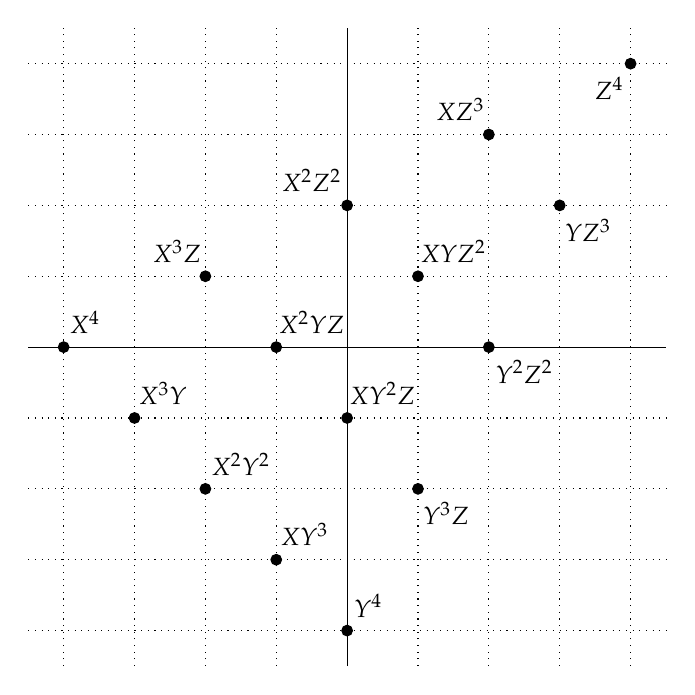
\begin{tikzpicture}[scale=0.9]
\foreach \x in {1, ..., 4} {
\draw[dotted] (-4.5, \x) -- (4.5,\x);
\draw[dotted] (-4.5, -\x) -- (4.5,-\x);
\draw[dotted] (\x, -4.5) -- (\x, 4.5);
\draw[dotted] (-\x, -4.5) -- (-\x, 4.5);
}
\draw (-4.5,0) -- (4.5,0);
\draw (0,-4.5) -- (0,4.5);
\filldraw (-4,0) circle [radius=0.075];
\filldraw (-3,-1) circle [radius=0.075];
\filldraw (-2,-2) circle [radius=0.075];
\filldraw (-1,-3) circle [radius=0.075];
\filldraw (0,-4) circle [radius=0.075];
\filldraw (1,-2) circle [radius=0.075];
\filldraw (2,0) circle [radius=0.075];
\filldraw (3,2) circle [radius=0.075];
\filldraw (4,4) circle [radius=0.075];
\filldraw (-2,1) circle [radius=0.075];
\filldraw (0,2) circle [radius=0.075];
\filldraw (2,3) circle [radius=0.075];
\filldraw (0,-1) circle [radius=0.075];
\filldraw (-1,0) circle [radius=0.075];
\filldraw (1,1) circle [radius=0.075];

\begin{small}
\draw (-3.7,0.35) node {$X^4$};
\draw (-2.6,-0.65) node {$X^3Y$};
\draw (-1.5,-1.65) node {$X^2Y^2$};
\draw (-0.6,-2.65) node {$XY^3$};
\draw (0.3,-3.65) node {$Y^4$};
\draw (0.5,-0.65) node {$XY^2Z$};
\draw (-0.5,0.35) node {$X^2YZ$};
\draw (1.5,1.35) node {$XYZ^2$};
\draw (1.4,-2.35) node {$Y^3Z$};
\draw (-2.4,1.35) node {$X^3Z$};
\draw (2.5,-0.35) node {$Y^2Z^2$};
\draw (-0.5,2.35) node {$X^2Z^2$};
\draw (3.4,1.65) node {$YZ^3$};
\draw (1.6,3.35) node {$XZ^3$};
\draw (3.7,3.65) node {$Z^4$};
\end{small}
\end{tikzpicture}
\caption{Weights for plane quartics.}
\end{figure}
% continuing

Then semistable monomials are given by sweeping out a line through the origin and seeing which monomials lie on one side. For example considering the line $y = -x$, the allowable monomials are $x^4, x^3 y, x^2 y^2, xy^3, y^4, x^3z, x^2yz, xy^2z,y^3z$. If we have such a curve $F$, then if we set $z=1$, the point $[0:0:1]$ has multiplicity at least $3$.

The next option is to include $x^4$ but not $y^4$ or $z^4$. One of the choices gives us the monomials $x^4, x^3 y, x^2 y^2, xy^3, x^3 z, x^2yz, x^2z^2$, and thus the curve is reducible.

Now we will consider points in projective space. We will construct $(\P^n)^m \sslash SL_{n+1}$. We will choose the line bundle $L = \mc{O}(k_1, \ldots, k_m)$. We know that $L$ is ample if and only if $k_i > 0$ for all $i$. We say that $k = (k_1, \ldots, k_m)$ is \textit{democratic} if $k_1 = \cdots = k_m$.\footnote{We would like to avoid Orwell's result that all points matter, but some points matter more than others.}

Choosing a $1$-PS with weights $q_0 \geq \cdots \geq q_n$, fix $P = (p_1, \ldots, p_m) \in (\P^n)^m$. Writing $p_i = [a_{i0}, \ldots, a_{i1}, \ldots, a_{iv_i}, 0, \ldots, 0]$ with $v_i \neq 0$, we see that 
\[ \mu^{L_k}(P, \lambda) = - \sum_{i=1}^m k_i qv_i. \]
Using some basic manipulation, this becomes
\[ \mu^{L_k}(P, \lambda) = -q_n \sum_{i=1}^m k_i + \sum_{j=0}^{n-1} \sum_{i=1}^m k_i \mathbb{1}_{\qty{p_i \in E_j}} ( q_{j+1} - q_j ). \]

\begin{thm}(\textbf{D}, Theorem 11.1)
    A point $P \in X^{ss}(L_k)$ if and only if for all $w \subseteq \P^n$,
    \[ \sum_{i, P_i \in w} k_i \leq \frac{\dim W + 1}{n+1} \sum_{i=1}^m k_i. \]
\end{thm}

\begin{proof}
    Suppose $q_0 = \cdots = q_s = n-s$ and $q_{s+1} = \cdots = q_n = -(s+1)$. The other direction is similar. We will neglect all of the explicit computations.
\end{proof}

\chapter{Morena (Oct 30): GIT and Moduli Problems}%
\label{sec:morena_oct_30_git_and_moduli_problems}

\section{Moduli Problems}%
\label{sec:moduli_problems}

One of the central problems in algebraic geometry is to classify various geometric objects: curves, schemes, sheaves. We want to find a space such that $M(K)$ is in bijection with isomorphism classes of our objects. However, this is trivially solved by taking a disjoint union of points, so we need a stronger notion of moduli problem. This is given by a functor
\[ M \colon (\ms{Sch}/S)^{\mr{op}} \to \ms{Set} \]
that sends a scheme $T$ to the set of families of objects over $T$.

\begin{exm}
    Consider the Hilbert functor $\mr{Hilb}_{M/R}$ that sends a scheme $S$ to 
    \[ \qty{X \subset M_S \mid X \to S \text{ flat and finitely presented}}. \]
\end{exm}

\begin{thm}
    The Hilbert functor is represented by a quasi-projected scheme.
\end{thm}

\begin{exm}
    Consider the functor $\P^n_{\Z}$ that sends
    \[ X \mapsto \qty{\mc{L}, s_1, \ldots, x_n \mid \mc{L} \in \Pic X, s_0, \ldots, s_n \in \mc{L}(X) \text{ generate X} }. \]
    This functor is represented by the scheme $\P^n$.

    Recall that there is a functor $\A^{n+1} \setminus 0 \to \P^n$. Then $X \to \A^{n+1} \setminus 0$ is the same thing as specifying $n+1$ sections of basepoint-free line bundle. For $U \subset X$ such that $\eval{\mc{L}}_U = \eval{\mc{O}}_U$, we obtain sections 
    \[ \qty( \frac{s_0}{t}, \ldots, \frac{s_n}{t} ) \colon U \to \A^{n+1} \setminus 0 \to \P^n. \]
    Because projective space does not see constants, we see that these maps glue and we obtain a global map.

    Conversely, consider $X \xrightarrow{i} \P^n$ and take the sections $i^*x_1, \ldots, i^* x_n \in i^* \mc{O}(1)$. These do not simultaneously vanish, so we obtain an invertible sheaf with generating sections.
\end{exm}

An obstruction to the solution of a moduli problem is the existence of nontrivial automorphisms. Suppose we want to classify vector bundles with rank $r$ over an algebraically closed field $k$. Call this functor
\[ B_r(X) = \qty{\text{vector bundles of rank $r$ over $X$}}. \]
If $Y$ represents this functor, then a curve with nontrivial vector bundle is a map $C \to Y$. Then given a cover $\qty{U_i}$ of $C$ by affines, then any vector bundle $\mc{V}$ is trivial when restricted to $U_i$. But then the trivial bundle is a closed point $y \in Y(k)$, and so if we attempt to glue the maps $U_i \to y \to Y$, then we obtain the map $C \to y \in Y$ and thus $\mc{V}$ must have been trivial in the first place. Therefore, there is no fine moduli space.

The next moduli problem we will consider is the moduli problem $M_{1,1}$ of elliptic curves over $k$. These are curves of genus $1$ with one marked point. To generalize this to families, we will take
\[ S \mapsto \qty{(f \colon E \to S, e \colon S \to E) \mid \text{$f$ smooth proper, $e$ section of $f$, $E_{\ol{s}}$ is an elliptic curve over $k(\ol{s})$}}. \]
Then a morphism $(a,b) \colon (S,E,e) \to (S',E',e')$ is a cartesian diagram
\begin{equation*}
\begin{tikzcd}
    E \arrow{r} \arrow{d} & E' \arrow{d} \\
    S \arrow{r} & S'
\end{tikzcd}
\end{equation*}
that commutes with the sections $e,e'$. Here, the criterion of being Cartesian means that defining the functor on morphisms is well-defined, because pullbacks are unique.

\section{Dealing with Nontrivial Automorphisms}%
\label{sec:dealing_with_nontrivial_automorphisms}


Unfortunately, there are nontrivial automorphisms of elliptic curves. Over $\C$ (or any algebraically closed of characterstic $p \neq 2,3$), we can write elliptic curves with the equation $y^2 = x(x-1)(x-\lambda)$. We then have an action of $S_3$ on $\Spec \C[t]_{(t(1-t))}$, where we have
\[ (\alpha, \lambda) \mapsto \frac{\alpha(\lambda) - \alpha(0)}{\alpha(1) - \alpha(0)}. \]
Then the orbit of $\lambda$ is the set 
\[ \qty{ \lambda, \frac{1}{\lambda}, \frac{1}{1-\lambda}, \frac{\lambda}{1-\lambda}, 1-\lambda, \frac{1- \lambda}{\lambda} }. \]
Generically, this has six points, but sometimes there are fewer (for example $\lambda = -1)$. Then we have the $j$-invariant
\[ j(\lambda) = 2^8 \frac{(\lambda^2 - \lambda + 1)^3}{\lambda^2(\lambda - 1)^2}, \]
and when $\lambda, \lambda'$ are in the same orbit, we have $j(\lambda) = j(\lambda')$. If we solve for $j(x) = j(\lambda)$, we obtain a polynomial of degree $6$, and thus generically there are six roots. Then we can see that all solutions belong to the orbit of $\lambda$. Therefore, we have
\[ \Spec (\C[t]_{(t(1-t))})^{S_3} = \Spec \C[j] \simeq \A^1_{\C}. \]
This discussion can be found in more detail in Hartshorne, Chapter 3, Section 4. We then see that $E \simeq E'$ if and only if $j(E) = j(E')$. Therefore, we have a bijection $M_{1,1}(\C) \simeq \A^1(\C)$. In fact, Silverman proves this identity for all fields.

However, we can show that $M_{1,1}$ has no fine moduli space. Consider the elliptic curves $Y^2Z = X^3 + tZ^3$ and $Y^2Z = X^3+tZ^3$ over $\C(t)$. We see that $E$ and $E'$ are not isomorphic at the level of $\C(t)$-points because $\C(t)$ contains no roots of $t$. However, if we base change to $\C(t^{1/6})$, then we obtain an isomorphism of the two curves by
\[ (X,Y,Z) \mapsto (t^{1/3}X, t^{1/2}Y, z). \]
This gives us a contradiction because for any field extension $L/K$ and scheme $X$, we have $X(K) \subset X(L)$.

There are two ways to resolve this problem of nontrivial isomorphisms:

\subsection{Stacks}%
\label{sub:stacks}

    We will in some sense, allow automorphisms. We can enlarge the category of schemes to algebraic spaces or stacks, in which we can restate the same problem. However, if we work with stacks, we will have to consider functors valued in the $2$-category of groupoids. For a functor $M \colon \ms{Sch}/S^{\mr{op}} \to \ms{Set}$, we will consider the functor
        \[ \mc{M} \colon \ms{Sch}/S^{\mr{op}} \to \ms{Gpd}, (T \to S ) \mapsto \mc{C}, \]
        where $\mc{C}$ is the category with objects the geometric objects over $T$ and morphisms the $T$-morphisms of such objects. The study of such things often becomes very topological. For elliptic curves, we can also rigidify our elliptic curves, we obtain a functor $R_{\mr{ell}} \colon \ms{Sch}/S^{\mr{op}} \to \ms{Set}$. This can then be represented by a scheme.

        In this case, a rigidified elliptic curve is an elliptic curve with nowhere vanishing section $\alpha \in H^0(E, \Omega_{E/S})$. Then automorphisms of rigidified elliptic curves are always trivial. Then writing $E$ in Weierstrass form, any map $E \to E'$ over $\Spec R$ extends to a map $\P^2 \to \P^2$. This is represented by a matrix 
        \[ A = \mqty(\dmat{u^2, u^3, 1}), \]
        where $u \in R^{\times}$. Then we can find a global nowhere vanishing section $\omega = \frac{Z}{2Y} d\qty(\frac{X}{Z})$. If $A$ preserves $\omega$, we see that
        \[ \omega = \frac{Z}{2u^3Y} d\qty(\frac{u^2X}{Z}) \]
        and thus $u = 1$. Thus we have killed all automorphisms. In fact, $R_{\mr{ell}}$ is represented by an affine scheme $\Spec \Z[a_4, A_6]_{\Delta}$, where $\Delta$ is the discriminant. Note here that $a_4, a_6$ are here because under $A$ an automorphism, we make the substitution $X = u^2 X, Y = u^3Y$, and $a_4, a_6$ become $u^4 a_4, u^6 a_6$. 
        
        Now consider the action of $\G_m$ on $R_{\mr{ell}}$ that scales the holomorphic $1$-form by $\frac{1}{\mu}$ (weight $-1$). Then we can define the morphism $R_{\mr{ell}} \xrightarrow{\pi} M_{1,1}$ that simply forgets $\omega$. Then we can define a quotient $R_{\mr{ell}} / \G_m$ and this gives a map to $M_{1,1}$. In this case, this is not a scheme, so we should really write the quotient \textbf{stack} $[R_{\mr{ell}} / \G_m]$.

    \subsection{Coarse Moduli}%
    \label{sub:coarse_moduli}
    
    
    Some of us are plebs who can only think about schemes.\footnote{This comment was added by the note-taker.} We will loosen our requirement for representability and find a scheme which approximates the problem as well as possible. We say a scheme $X$ \textit{coarsely represents} $M$ if 
    \begin{enumerate}
        \item $\psi \colon M \to h_X$ is a bijection over algebraically closed fields.
        \item For all $\phi \colon M \to h_Y$ such that the first item holds, there exists a unique morphism $h_X \to h_Y$ that makes the diagram commute.
    \end{enumerate}

    There are several problems that may arise: either $X$ may be non-separated or it may have infinitely many components. In addition, even if $X$ is separated with finitely many components, it may not be a scheme. Here are some more problems:
    \begin{enumerate}
        \item If we take varieties with no extra data, we run into the problem of having many automorphisms. This can be fixed by adding the datum of a polarization, which rigidifies the problem. For $X/k$ proper, we can consider $\Pic^{\tau}(X) \subset \Pic X$ composed of line bundles such that $\mc{L}^m \in \Pic^0(X)$ for some $m$. Then an \textit{inhomogeneous polarization} is a coset formed by ample line bundles. For example, for $C \to k$ of genus at least $2$, the dualizing sheaf $\omega_C$ is ample, and then $\omega_C^3$ is very ample.  
    \end{enumerate}
In Mumford, if we follow references [29] and [135], we see that requiring smoothness makes the the coarse moduli space $X$ is separated and has finitely many components. However, smoothness is an open condition, so our moduli space will not be compact and thus will not have a good intersection theory. For example, take the intersection of two lines in the plane. Two parallel lines do not intersect in $\A^2$, but they do intersect at infinity in $\P^2$. Thus, we will define the space $\ol{M}_g$, which is the moduli space of \textit{stable curves}, where we allow nodes. In stack form, this becomes a proper Deligne-Mumford stack.. 

\chapter{Morena (Nov 6): GIT and Coarse Moduli Problems (Part 2)}%
\label{cha:morena_nov_6_git_and_coarse_moduli_problems_part_2_}

\section{Moduli of Curves}%
\label{sec:moduli_of_curves}

Recall that the functor $M_g$ sends a scheme $S$ to the set of isomorphism classes of smooth curves of genus $g$ over $S$. More precisely, these are flat and proper morphisms $f \colon C \to S$ such that geometric fibers are curves of genus $g$. Then recall that morphisms are given by cartesian diagrams. We will now rigidify this problem to find a coarse moduli space. 

\begin{thm}[Olsson, Lemma 8.4.6]
    Let $f \colon C \to S$ be a curve of genus $g \\geq 2$. Then consider $\omega_f = \Omega^1_{C/S}$. 
    \begin{enumerate}
        \item $f_* \omega_f^3$ is locally free of rank $5g-5$.
        \item The map $f^* f_* \omega_f^{\otimes 3} \to \omega_f^{\otimes 3}$ is surjective and $C \hookrightarrow \P(f_* \omega_f^{\otimes 3})$ is a closed embedding. Here, $\P(\text{vector bundle})$ is simply the relative Proj of the sheaf over $S$.
    \end{enumerate}
\end{thm}

\begin{defn}
    Define the functor $H_3 \colon \ms{Sch}/\Z^{\mr{op}} \to \ms{Set}$ of rigidified smooth curves by
    \[ H_3(S) = \qty{ f \colon C \to S, \P(\sigma) \colon \P(f_* \omega_f^{\otimes 3}) \to \P_S^{5g-6} ) } / \sim, \]
    where the map of projective spaces is an $S$-isomorphism. Here, morphisms are cartesian squares
    \begin{equation*}
    \begin{tikzcd}
        C \arrow{r}{b} \arrow{d}{f} & C' \arrow{d}{f'} \\
        S \arrow{r}{a} & S'
    \end{tikzcd}
    \end{equation*}
    such that
    \begin{equation}
        \label{eqn:largerect}
    \begin{tikzcd}
        C \arrow{d}{b} \arrow[hookrightarrow]{r} & \P(f_* \omega_f^{\otimes 3}) \arrow{r}{\P(\sigma)} \arrow{d}{\ol{b}} & \P_S^{5g-6} \arrow{r} \arrow{d}{\ol{a}} & S \arrow{d}{a} \\
        C' \arrow[hookrightarrow]{r} & \P(f'_* \omega_{f'}^{\otimes 3}) \arrow{r}{\P(\sigma')} & \P_S^{5g-6} \arrow{r} & S
    \end{tikzcd}
    \end{equation}
    commutes and the right square is commutative.
\end{defn}

Fortunately, there are no nontrivial automorphisms, so there is hope that this functor is represented by a scheme.

\begin{thm}
    The functor $H_3$ is represented by a locally closed subscheme of $\ul{\mr{Hilb}}_{\P^{5g-6}}^{p(t)}$, where 
    \[ p(t) = \chi(\omega_f^{\otimes 3t}) = \deg(\omega_f^{\otimes 3t}) + 1 - g = (6g-6)t + 1-g\]  
    by the Riemann-Roch theorem. The embedding $H_3 \to \ul{\mr{Hilb}}^p$ is given by
    \[ (f \colon C \to S, \P(\sigma)) \mapsto C \hookrightarrow \P(f_* \omega_f^{\otimes 3}) \xrightarrow{\P(\sigma)} \P_S^{5g-6}. \]
\end{thm}

Now note that $\mr{Hilb}^{p(t)}$ is a projective scheme. Then the identity map corresponds to the universal closed subscheme $\mf{Z} \hookrightarrow \P^{5g-6}_{\mr{Hilb}}$. However, $\mc{Z} \to \mr{Hilb}$ is not smooth (but it is flat and proper), so we can take $W \subset \mc{Z}$ the non-smooth locus, so then we can take $\mr{Hilb} \setminus f(W)$ parameterizing smooth subschemes.

Now to impose geometrically connected fibers, we use Stein factorization (Stacks Project, 37.48.5). This says many things, but what we need is that if we have $f \colon X \to S$ proper, then we can find $S' \to S$ such that $f'\colon X \to S'$ is proper and has geometrically connected fibers and such that $S' \to S$ is integral and is an isomorphism over an open subscheme of $S'$. This implies using the Hilbert polynomial that $\dim = 1$ and that the genus is $g$. Thus we have an open subscheme $H' \subset \mr{Hilb}$ parameterizing smooth curves.

Now the identity $H' \to H'$ gives a universal smooth curve
\begin{equation*}
\begin{tikzcd}
    C' \arrow[hookrightarrow]{r} \arrow{dr} & \P_{H'}^{5g-6} \arrow{d} \\
                                            & H'.
\end{tikzcd}
\end{equation*}
To recover $\P(\sigma)$, we need this to factor through $\P(f_* \omega_f^{\otimes 3})$. Therefore, we need the pushforwards of $\Omega_{C'/H'}^{\otimes 3}$ and $i^*(\mc{O}_{\P^{5g-5}}(1))$ to pushforward to the same sheaf under $f'_*$. Here, the two sheaves give morphisms $H' \rightrightarrows \Pic_{C'/H'}$ and the square
\begin{equation*}
\begin{tikzcd}
    H_2 \arrow{r} \arrow{d} & H' \arrow{d} \\
    \Pic_{C'/H/} \arrow{r}{\Delta} & \Pic_{C'/H'} \times_{H'} \Pic_{C'/H'}
\end{tikzcd}
\end{equation*}
is cartesian. Then $\Pic$ is separated, so $\Delta$ is a closed embedding. Thus we have a closed subscheme $H_2 \subset H'$. Now we ask for a surjective map
\[ H^0(H', f'_* i^* \mc{O}(1)) \otimes \mc{O}_{H'} \to f_* \omega_f^{\otimes 3}. \]
This is the same as the cokernel vanishing, so now we have $H_3 \subset H_2$ an open subscheme. This is also Proposition 5.1 in Mumford.

Now we have shown that the rigidified moduli problem $H_3$ is representable. Then we consider the map $\pi \colon H_3 \to M_g$ that forgets $\P(\sigma)$, and so we have an action of $PGL_{5g-5}$ on $H_3$ by postcomposition with $\P(\sigma)$. Now we define $M_g' = H_3 / PGL = (S \mapsto H_3(S) / PGL(S))$. Then we have a map $H_3 / PGL \xrightarrow{I} M_g$ compatible with $\pi$. Here $I$ is a ``principal bundle'' and so $I$ is injective and locally surjective, which means that for all $S$ there exists $\alpha \in M_g(S)$ and Zariski cover $\qty{S_i \to S}$ such that $\alpha|_{S_i} \in \Im(I)$.

Then checking $\pi([f, \P(\sigma)]) = \pi([f', \P(\sigma')])$, we use the large commutative diagram (\ref{eqn:largerect}) to see that $f,f'$ are related by some element of $PGL$. Then there exists a geometric quotient $H_3 / PGL$ and this is a coarse modulu space for $M_g$. Thus we have a bijection between maps $M_g \to N$ and $PGL$-invariant maps $H_3 \to N$. This is equivalent to the orbits of $H_3(\Omega)$ to be bijective with $N(\Omega)$, where $N = H_3 / PGL$.

Now recall from Theorem 3.4.5 that if $X/k$ is of finite and $G$ is a reductive group with $\mc{L} \in \Pic^G(X)$, then there is a universal categorical quotient of $X^{\mr{ss}}(\mc{L})$ and a uniform geometric quotient of $X^s(\mc{L})$ (in characteristic $0$, uniform is upgraded to universal). Now we want to express $H_3$ as the locus of stable points of something, and in particular as $X^s_{(0)}(\mc{L})$.

To do this, we will introduce the Chow scheme. The Chow variety $\mc{C}_{n, r, d}$ parameterizes subvarieties of $\P^n$ of dimension $r$ and degree $d$. This is defined by
\[ X \mapsto \Gamma = \qty{(x, \mu_0, \ldots, \mu_r) \mid x \in \mu_i \text{ for all }i = 0, \ldots, r} \subset X \times (\P^n)^{r+1}. \]
Then projecting $\Gamma$ down to $(\P^n)^{r+1}$, we obtain a hypersurface defined by the \textit{Cayley form} $F_X$. Then the coefficients of $F_X$ map to $\mc{C}(X) \in \P^{\nu}$. 

Now we have a map $\phi \colon H_3 \to \mc{C}_{5g-6, 1, 6g-6}$. Over $k$, we use a push-pull with respect to 
\begin{equation*}
\begin{tikzcd}
    & \mc{X} \arrow{dl}{p_1} \arrow{dr}{p_2} \\
    \P^n & & \P^n \times \P^n
\end{tikzcd}
\end{equation*}
where $\mc{X}$ is defined by first defining $H = \sum x_i \otimes U_i \subset \P^n \times \P^m$, then pulling considering the maps $p_{12}, p_{13} \colon \P^n \times \P^n \times \P^n \to \P^n \times \P^n$, and taking $\mc{X} = p_{12}^{-1}(H) \times p_{13}^{-1}(H)$.

Now recall from Proposition 1.14 of Mumford that $\ol{X}^{ss}(\ol{\mc{L}}) = \ol{X^{ss}(\mc{L})}$ and similarly for the stable locus. Thus we can reduce to the case where $k$ is algebraically closed, and by Proposition 1.18 in Mumford, if $f \colon X \to Y$ is $G$-equivariant, then $f$ is quasi-affine. Thus $f^{-1}(Y_{(0)}^s(\mc{L})) \subseteq X_{(0)}^s(f^* \mc{L})$. Then by Theorem 6.2 in SGA 8, an injective morphism of finite type is quasi-affine. If we require that $f$ is finite, $X$ is proper, and $\mc{L}$ is ample, the inclusion becomes an equality by Proposition 1.19 in Mumford.

Now recall that we have $\phi \colon H_3 \to \mc{C}_{5g-6, 1, 6g-6}$. Then $\phi$ is quasi-affine and $\phi^{-1}(\mc{C}_{(0)}^s ( \mc{O}_{\mc{C}}(1) )) \subset (H_3^s)_{(0)}(\phi^* \mc{O}_{\mc{C}}(1))$. Then by Theorem 4.5 of Mumford, we use the Hilbert-Mumford stability criterion to see that for any smooth curve $\gamma$, the point $\mc{C}(\gamma)$ is stable if
\begin{enumerate}
    \item $\gamma$ is not contained in a hyperplane.
    \item $\gamma$ is defined by a complete linear system.
    \item $g \geq 1$ and $\deg \gamma \geq 3g$. This is equivalent to $g \geq 2$.
\end{enumerate}
Thus the image of $\phi$ is contained in the properly stable locus and thus we have $H_3$ is equal to the properly stable locus. Thus we obtain a geometric quotient.

\chapter{Kuan-Wen (Nov 13): GIT and the moment map}%
\label{cha:kuan_wen_nov_13_git_and_the_moment_map}

\section{Moment maps}%
\label{sec:moment_maps}

Let $(X, \omega)$ be a symplectic manifold. Here, this means that $X$ is a smooth manifold and $\omega$ is a closed nondegenerate $2$-form on $X$. Now Let $K$ be a compact Lie group acting on $X$ symplectically, which means $k^* \omega = \omega$ for all $k \in K$. Define the Lie algebra of $K$ to be $\mf{k}$.

\begin{defn}
    The \textit{moment map} $\mu \colon X \to \mf{k}^*$ is a map which is
    \begin{enumerate}
        \item Equivariant. Here, we use the coadjoint action on $\mf{k}^*$.
        \item The map $\dd{\mu} \colon T X \to \mf{k}^*$ satisfies the identity
            \[ \dd{\mu}(x)(\xi) . a = \omega_x(\xi, a_x) \]
            for any $x \in X, a \in \mf{k}$ and $a_x = \eval{\dv{x} \exp(ta)x}_{t=0}$.
    \end{enumerate}
\end{defn}

Now we will discuss existence and uniqueness of the moment map. For uniqueness, we know that
\begin{enumerate}
    \item $\mu$ is unique up to addition of a constant in $\mf{k}^*$.
    \item If $K$ is semisimple, then the only fixed point of the coadjoint action is $0$, and thus $\mu$ is in fact unique.
    \item If we require $\int_X \mu \omega^n = 0$ for $X$ compact, then we obtain a unique moment map.
\end{enumerate}

Now we will discuss existence. The following result is from reference [723] of Mumford's book.

\begin{thm}[Marsden-Weinstein]
    If $K$ is semisimple, then the moment map $\mu$ exists.
\end{thm}

Next, it is known that if $H^1(X,\Q) = 0$ and $K$ is connected, then the moment map exists. If $K$ is a torus, this comes from a differential equation, but the obstruction comes from $H^1(X, \Q)$ and so we are fine here. In general, we have an exact sequence
\[ 0 \to \qty{\text{finite central}} \to \prod \qty{\text{semisimples}} \times \text{torus} \to K \to 0 \]
so by the previous discussion, we now have the existence of a moment map.

\begin{exm}
    Consider the standard action of $U(n+1)$ on $\P^n$. Then the mment map $\mu \colon \P^n \to \mf{u}(n+1)^*$ is given by
    \[ x \mapsto \mu(x) .a = \frac{\ol{x^*}^t a x^*}{2 \pi i \norm{x^*}^2} \]
    where $x^*$ is any lift of $x$ in $\C^{n+1}$. This is unique up the the addition of the trace map $\tr(-)$, which is the nontrivial fixed point of the coadjoint action. This follows from the fact that all characters of $U(n+1)$ are powers $\det^m \colon U(n+1) \to S^1$ of the determinant map. To see invariance, note that
    \[ \mu(kx).a = \frac{\ol{x^*}^t \ol{k}^t a k x^*}{2 \pi i \norm{x^*}^2} = \mr{Ad}^*(k) \mu(x).a. \]
    Using the Fubini-Study metric on $\P^n$ and the fact tha tthe action is transitive, we will compute at the point $[ 1:0:\cdots :0 ]$ with coordinates $[1:x^1:\cdots :x^n]$. Recall that the Fubini-Study form is given by
    \[ \omega_{\mr{FS}} = \frac{i}{2\pi} \sum_j \dd{x}^j \wedge \dd{\ol{x}}^j. \]
    Now we can directly compute
    \begin{align*}
        \dd{\mu} &= \dd{\qty(\frac{\ol{x^*}^t a x^*}{2 \pi i \norm{x^*}^2})} \\
                 &= \frac{i}{2\pi} \sum \ol{a}_j \dd{x^j} - a_j \dd{\ol{x}}^j \\
                 &= \omega_{\mr{FS}}(-,a).
    \end{align*}
    This gives the desired result.
\end{exm}

Now suppose $X \subset \P^n$ and $K$ acts on $X$ with an action induced from a linear action on $\P^n$. Then we can assume that $K$ acts unitarily, so then se can write the moment map as
\[ X \hookrightarrow \P^n \xrightarrow{\mu} \mf{u}(n+1)^* \to \mf{k}^*. \]
This can be written explicitly as
\[ \ol{\mu}(x).a = \frac{\ol{x^*}^t \rho_*(a)x^*}{2\pi i \norm{x^*}^2} \]
where $\rho \colon K \to U(n+1)$ is the linear action.


We will now discuss quotients in the symplectic category.
\begin{thm}[Marsden-Weinstein]
    Let $K$ act on $(X, \omega)$ and $\mu \colon X \to \mf{k}^*$ be the moment map. Let $\eta \in \mf{k}^*$ be a fixed point of the coadjoint action. If $K$ acts freely and properly on $\mu^{-1}(\eta)$, then the quotient $\mu^{-1}(\eta)/K$ is a symplectic manifold of dimension $\dim X - 2 \dim K$. If $\iota \colon \mu^{-1}(\eta)$ is the inclusion and $\pi$ is the projection, then we have the identity $\pi^*\omega^{\mr{red}}  = \iota^*\omega$. If $\eta$ is not fixed, we can replace $K$ by the stabilizer of $\eta$.
\end{thm}

\begin{proof}
    We have the equality
    \[ \ker \dd_x{\mu} = T_x(K \cdot x)^{\omega_X} \coloneqq \qty{v \in T_x X \mid \omega_x(\eta, v) = 0 \text{ for all } \eta \in T_(K \cdot x)}. \]
    This comes from the differential equation in the definition of the moment map, and then we also have
    \[ \Im \dd_x {\mu} = \mr{Ann}(\mf{k}^*) = \qty{\eta \in \mf{k}^* \mid \eta \cdot A = 0 \text{ for all }A \in \mf{k}_x}. \]
    To get the dimension equality, we have a short exact sequence for any $W \subseteq T_x X$ given by
    \[ 0 \to W^{\omega_x} \to T_x X \to W^* \to 0 \]
    and thus $\dim T_x X = \dim W + \dim W^{\omega_x}$. Now we replace $W$ with $T_x(K\cdot x)$ to obtain the desired result. On the other hand, we also have
    \[ \dim \mr{Ann}(\mf{k}_x) = \dim \mf{k} - \dim \mf{k}_x = \dim T_x X - \dim T_x(K \cdot x)^{\omega_x} = \dim \Im \dd{x} \mu. \]
    By these computations, we know that $\eta$ is a regular value if and only if the action of $K$ on $\mu^{-1}(\eta)$ is locally free.

    Now $T_x(K \cdot x)$ is an isotropic subspace of $T_x X$ because we have
    \[ T_x(K \cdot x) \subset T_x \mu^{-1}(\eta) = T_x(K \cdot x)^{\omega_x}. \]
    Next, for isotropic subspaces $I$ of $(V, \omega)$, there is a symplectic form induced by $\omega$ on $I^{\omega} / I$. This gives a symplectic form on $T_x(K \cdot x)^{\omega_x} / T_x(K \cdot x) = T_x \mu^{-1}(\eta) / T_x(K \cdot x)$, and so we have a symplectic form on the quotient.

    Finally, to prove closedness of this form, this follows from the fact that 
    \[ \pi^* \dd{\omega^{\mr{red}}} = \dd{(\pi^* \omega^{\mr{red}})} = \dd{(\iota^* \omega)} = \iota^* \dd{\omega} = 0 \]
    and the fact that $\pi^*$ is injective.
\end{proof}

\section{Comparison of symplectic quotients and GIT quotients}%
\label{sec:comparison_of_symplectic_quotients_and_git_quotients}

Now let $G$ is reductive with a linear action $\rho \colon G \to GL(n+1)$ such that $G$ acts on some projective variety $X \subseteq \P^n$. Now let $K \subset G$ be a maximal compact subgroup. 

\begin{thm}
    \begin{enumerate}
        \item A point $x \in X$ is semistable if and only if $\ol{O_G(x)} \cap \mu^{-1}(0) \neq \emptyset$.
        \item There is an inclusion $\mu^{-1}(0) \hookrightarrow X^{\mr{ss}}$ (by Proposition 2.2 in Mumford). This induces a homeomorphism $\mu^{-1}(0)/K \simeq X \sslash G$ with the GIT quotient.
    \end{enumerate}
\end{thm}

\begin{proof}
    First, for all $v \in \C^{n+1}$, define $p_v(g) = \norm{gv}^2$. Then from Kempf-Ness (reference [175] in Mumford), we have
    \begin{enumerate}[label=(\roman*)]
        \item All critical points of $p_v$ are minima.
        \item If $p_v$ attains a minimum, it does so on exactly one double coset in $K \backslash G / G_v$.
        \item $p_v$ attains a minimum if and only if the orbit of $v$ is closed in $\C^{n+1}$.
    \end{enumerate}
    Also, because we can write the moment map explicitly, we have $\dd{p}_{x^*}(g) = 0$ if and only if $\mu(gx) = 0$. Finally, we know that if $O_G(x^*)$ is closed in $\C^{n+1}$, then $x$ is semistable and $O_G(x)$ is closed in $X^{\mr{ss}}$. To prove the second part, if $y \in \ol{O_G(x)} \cap X^{ss}$, then there exists $f$ invariant such that $y \in X_f$. This means $x \in X_f$, so we can choose $x^*, y^*$ such that $f(x^*) = f(y^*) = 1$. Multiplying by roots of unity, we may assume that $y^* \in \ol{O_G(x^*)} = O_G(x^*)$. Projecting down, we have $y \in O_G(x)$.

    Using all of these observations, we can prove the two parts of the theorem.
    \begin{enumerate}
        \item If $x \in X^{\mr{ss}}$, then $\ol{O_G(x)} \subset \C^{n+1} \setminus \qty{0}$ contains some closed orbit $O_G(y)$. This implies that $\ol{O_G(x)} \cap \mu^{-1}(0) \neq \emptyset$. The converse simply follows from the observations and Proposition 2.2 in Mumford.
        \item We know $\mu^{-1}(0)/K \to X \sslash G$ is a continuous map from a compact space to a Hausdorff space. It suffices to show taht this is a bijection. Then recall that $X^{\mr{ss}} \xrightarrow{\phi} X \sslash G$ satisfies the condition that $\phi(x) = \phi(y)$ if and only if their orbit closures intersect, so by the first part of this theorem, we have surjectivity.

            For injectivity, if $\mu(x) = 0 = \mu(y)$ but $x \notin O_K(y)$, then we know that $x \notin O_G(y)$ by the previous discussion, but also $O_G(x), O_G(y)$ are closed in $X^{\mr{ss}}$, which gives a contradiction. \qedhere
    \end{enumerate}
\end{proof}

We conclude with some remarks. It is easier to compute the cohomology of $\mu^{-1}(0) / K$ than it is to compute the cohomology of $X \sslash G$. To do this, if we consider the Morse function $f(x) = \norm{\mu(x)}^2$, where the norm comes from the Killing form, then we have a Morse stratification $\qty{C_{\beta, m}}$ and then we define the functions 
\[ p_t^K(X) = \sum t^i \dim H_K^i(X,\Q) = \sum_{\beta, m} t^{d(\beta, m)} p_t^K(C_{\beta, m}). \]
This allows us to compute the cohomology.








\end{document}
